\chapter{Related Works}
\label{cha:relatedworks}
Image-text alignment is a fundamental research topic in the inter-field of computer vision and natural language processing. There are many approaches proposed to associate images with textual attributes or vice versa. However, the fielded applications on bidirectional image sentence mapping appear to be relatively few, especially for multi-modal question answering. 

It has been suggested that this is due to the intense labour has been paid on annotating artworks for online digital artwork archives, automated image or sub-image with its textual attributes description could significantly improve the payoff. In this chapter we will survey and summarise the literature of image-text alignment and some proposed applications on multi-modal question answering.

The structure of this chapter is as follows. Section 2.1 discusses the history and some basic knowledge of image recognition. Section 2.2 discusses the preliminaries on deep learning and some mainstream object detection techniques. Section 2.3 explains the definition of image-text alignment and related proposed solutions on that task. Section 2.4 summarises this section.

\section{Image Recognition}
The history of research on image recognition stems from the 1960s when Marvin Minsky, also known as ``the father of Artificial Intelligence'' asked his student Gerald Sussman to ``connect a camera to a computer and do something with it'' \cite{hill}. But with minimal resource, this topic did not get enough attention at first. 

\subsection{Early Researches on Image Recognition}

After entering 1970s, the advent of modern electronic computers gives computers a chance to try to answer what they see through images. Researchers first tried to learn from the same way human look at things. It was generally believed that humans could see and understand things because they could observe things in 3-D with two eyes, which now seems rather absurd. Therefore, researchers believed that for a computer to understand the image it sees, it must first recover the three-dimensional structure of the object from its two-dimensional image. This is the so-called ``three-dimensional reconstruction'' method.

Another inspiration is that it was believed that people could recognise an object, for instance: an apple because people already have a priori knowledge: ``Apples are red, round, and smooth''. If a machine was also established with such a knowledge base, then it could match the images with its knowledge base, and potentially comprehend what it sees corresponding to what it already knew. This is the so-called ``a priori knowledge base'' method. However, this method can only extract very few basic features, which is not very practical.

By the 1990s, image processing hardware technology had made huge progress. Meanwhile, researchers began to design different algorithms: introduction of statistical methods and local feature descriptors, which led to more significant development of computer vision technology and started to be widely used in the industries. In the ``a priori knowledge base'' method, the shape, colour, surface texture, and other characteristics of objects are affected by the viewing angle and the observation environment, and they will change under different angles, different lights, and different occlusions. To solve that dilemma, the proposed new method judges things through identification of local features, and establish a local feature index on objects, which can be more accurately matched even if the perspective or observation environment changes.

After entering the $21^{st}$ century, computer vision develops rapidly thanks to the massive data brought by the rise of the Internet, the advent of digital cameras, and the widespread application of machine learning methods. In the past, many rule-based processing methods have been replaced by machine learning: machines automatically summarise the characteristics of objects from massive data then identify and classify. Many applications are emerging at this stage, including camera face identification, security face recognition and license plate recognition, etc. The accumulation of data has also produced many evaluation data-sets, such as official face recognition and face comparison recognition platforms: \textit{FDDB} and \textit{LFW}. One of the most famous ones is \textit{ImageNet} \cite{imagenet}, which contains 14 million labelled images divided into tens of thousands of categories.


\subsection{Image Recognition with Neural Networks}
After 2010, with the power of deep learning, computer vision technology has experienced explosive growth and industrialisation. With the adoption of neural networks, image recognition tasks can be achieved much more efficient and accurate. Figure \ref{fig:nnexample}. below gives us a straightforward illustration of how neural networks help with image recognition.

\begin{figure}[h!]
\centering
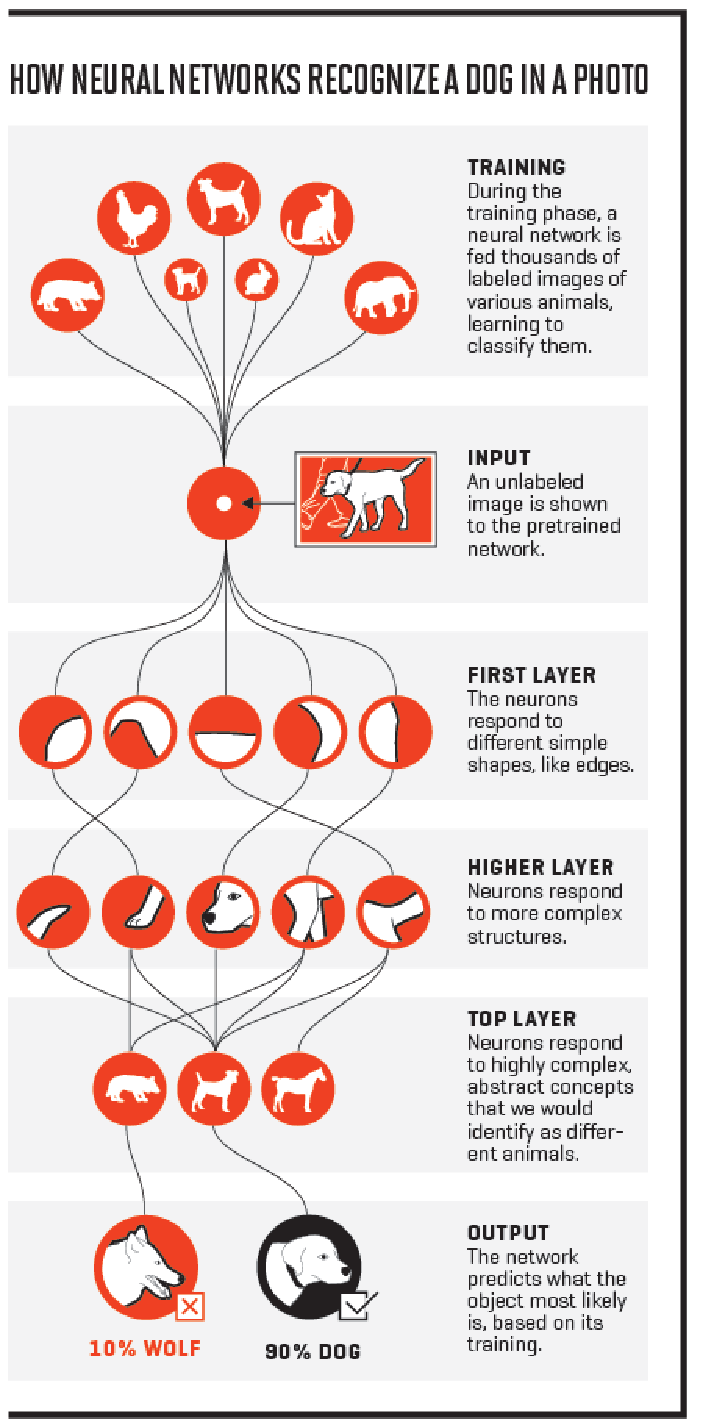
\includegraphics[width=0.4\textwidth]{nnexample.pdf}
\caption{How Neural Networks Performs an Image Recognition Task \cite{parloff_2019}}
\label{fig:nnexample}
\end{figure}

Next, we introduce deep neural networks and how neural networks can be adopted to solve object detection tasks, which is the core part of our project.

\section{Deep Learning and Object Detection}

Through deep neural networks, the accuracy of various types of visual recognition tasks has been dramatically improved. In the well-known computer vision competition ILSVR, the error rate of thousands of object recognition was as high as 25.8\% in 2011. After the introduction of deep learning in 2012, the error rates in the following four years reached 16.4\%, 11.7\%, and 6.7\%, 3.7\%, with significant breakthroughs. Now, face recognition can even achieve a false positive rate of less than one over a million.

Now we know that deep learning has several advantages on image processing and always surpasses other mainstream techniques. But what is deep learning? The following paragraphs give a brief idea of deep learning and how it works.

\subsection{Deep Learning}
In real life, human beings can often solve many problems by intuition. For example, when a human sees Figure \ref{fig:catanddog}. below, he or she can immediately know that there is a cat and a dog in the picture.

\begin{figure}[h!]
\centering
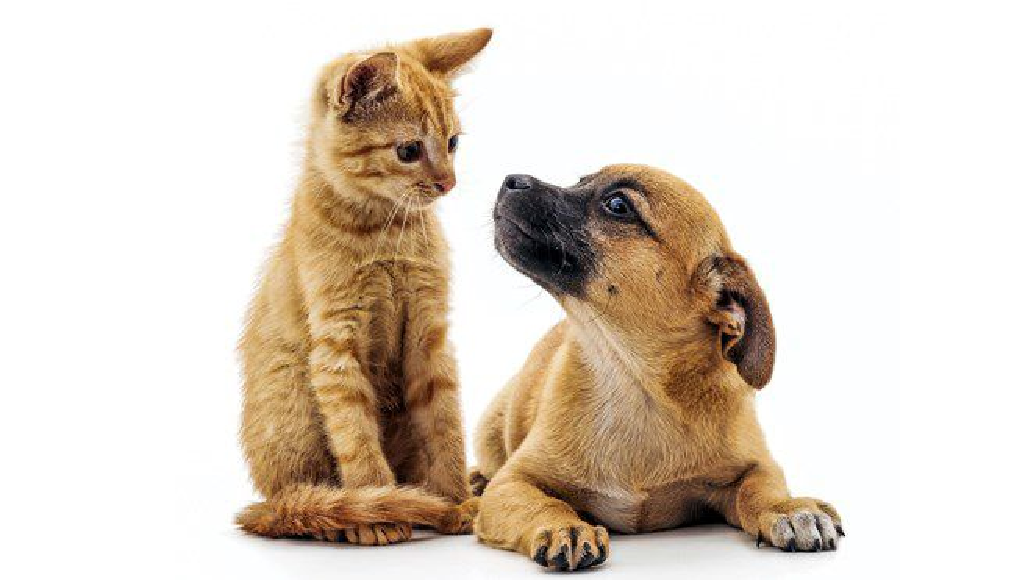
\includegraphics[width=0.4\textwidth]{catanddog.pdf}
\caption{Image of a Cat and a Dog}
\label{fig:catanddog}
\end{figure}

This may feel a natural task for human, but think about how do human know that there are a cat and a dog, but not two cats or two dogs instead? As human can differentiate these two from the picture at a glance, let's try to describe the appearance of cats and dogs. Taking the above picture as an example, we can describe the morphological characteristics of cats as follows: it has a round head, wide cheeks, wide ear roots, deep auricles, and rounded parts at the tip. For the dog in the picture above, its head is flat and wide; the ears are small and thin, the tips of the ears are slightly rounded, the dark apricot eyes, and short hair. Words ``broad cheeks'' and ``round ear tips'' often apply to cats and dogs, while the length of short hair and round ears cannot be quantified with a specific number. When we try to adopt a more specific description like ``dark apricot eyes'', a new problem arises: not all breeds of dogs have such characteristics, but we can still recognise them quickly at a glance.

In short, it is challenging to distinguish cats and dogs accurately with a few words or sentences, but this problem is often solved quickly and accurately by intuition. To solve these seemingly intuitive problems on computers, it is difficult to describe them with specific language or mathematical rules. This brought the invention of deep learning.

Deep learning is to let computers simulate human cognitive processes and learn from experience (also as known as ``intuition''). Make computers understand tasks using a hierarchical concept system like human while each concept is defined by some relatively more straightforward concepts: building simpler concepts to learn complex concepts. The word ``deep'' means more layers of learning system. 

Deep learning has a long and rich history. With the increasing amount of available training data and the continuous improvement of computer software and hardware, the scale of deep learning models has also increased to solve increasingly complex application problems, and the accuracy has continued to increase.



\subsection{Image Understanding}
How to retrieve information out from images that can be understood by a computer has always been the most discussed field of computer vision. Deep learning model have become a popular research area due to its powerful representation capabilities, coupled with the accumulation of data and advances in computing power.

But how to understand an image? There are three main levels according to the needs of subsequent tasks: classification, detection and segmentation. Figure \ref{fig:odsteps}. below provides an example how image understanding tasks can be performed \cite{ouaknine_2018}.

\begin{figure}[h!]
\centering
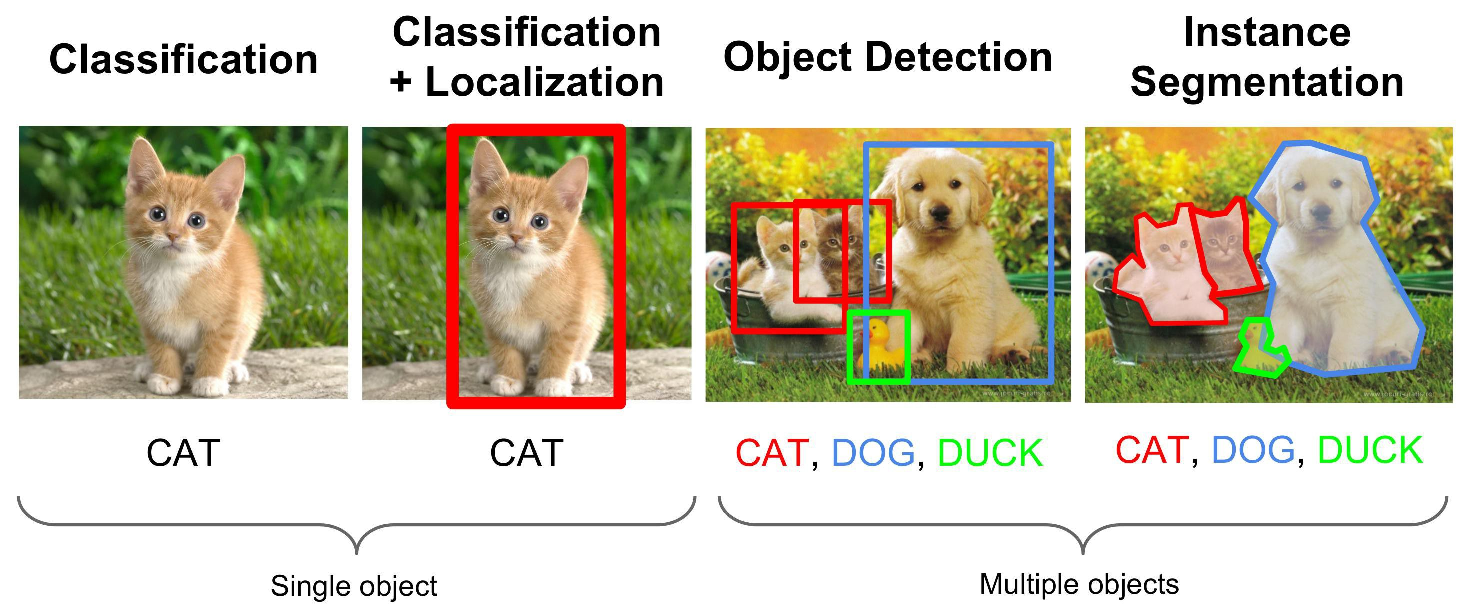
\includegraphics[width=0.7\textwidth]{dlstep.pdf}
\caption{Three Steps of Image Understanding \cite{ouaknine_2018}}
\label{fig:odsteps}
\end{figure}

\subsubsection{Classification}
Classification is the first task, is to structure an image into information of a certain category then describe it by a predetermined category (string) or instance ID. Classification task is the simplest and most basic image understanding task, and it is also the first task for deep learning models to achieve breakthroughs and achieve large-scale applications. In the application field, face recognition and scene recognition can be classified as classification tasks.

\subsubsection{Detection}
The classification task gives the content description of the entire picture, while the detection focuses on the specific object target, which requires the category information and position information of the target to be obtained at the same time. Comparing to the classification task, detection gives an understanding of both foreground and background of the image. To perform detection, we need to separate the interesting targets from the background and determine the description, i.e. category and location of this target. Therefore, the output of this detection model is a list, each item of the list uses a data set to give the category and position of the detected target, which is commonly represented by the coordinates of a rectangular detection frame.

\subsubsection{Segmentation}
Segmentation includes semantic segmentation and instance segmentation. The former is an extension of the previous background separation and requires the separation of image parts with different semantics, while the latter is an extension of the detection task and requires the outline of the target which is finer than the detection frame. Segmentation is a pixel-level description of an image. It gives meaning to each pixel category, i.e. instance and is suitable for understanding demanding scenes, such as the segmentation of roads and non-roads in driver-less technology.

\subsection{Object Detection}

After familiarised the steps of image understanding, in this section we focus on the second task: object detection, which is also the main task of our proposed work. The following paragraph will provide several mainstream models on solving object detection tasks.

\subsubsection{CNN}
First we start with introducing a series of commonly used models called convolutional neural networks (CNN). 

%convolution
\paragraph{Convolution Process}
The convolution process is based on a small matrix, that is, a convolution kernel. The pixel matrix of each layer mentioned above is continuously scanned in steps, the scanned number is multiplied by the number of the corresponding position of the convolution kernel, and then the sum is calculated. Each time you scan, you get a value, and after all the scans, a new matrix is generated. The following Figure \ref{fig:convolutionprocess} illustrates an example of convolution process in a CNN model:

\begin{figure}[h!]
\centering
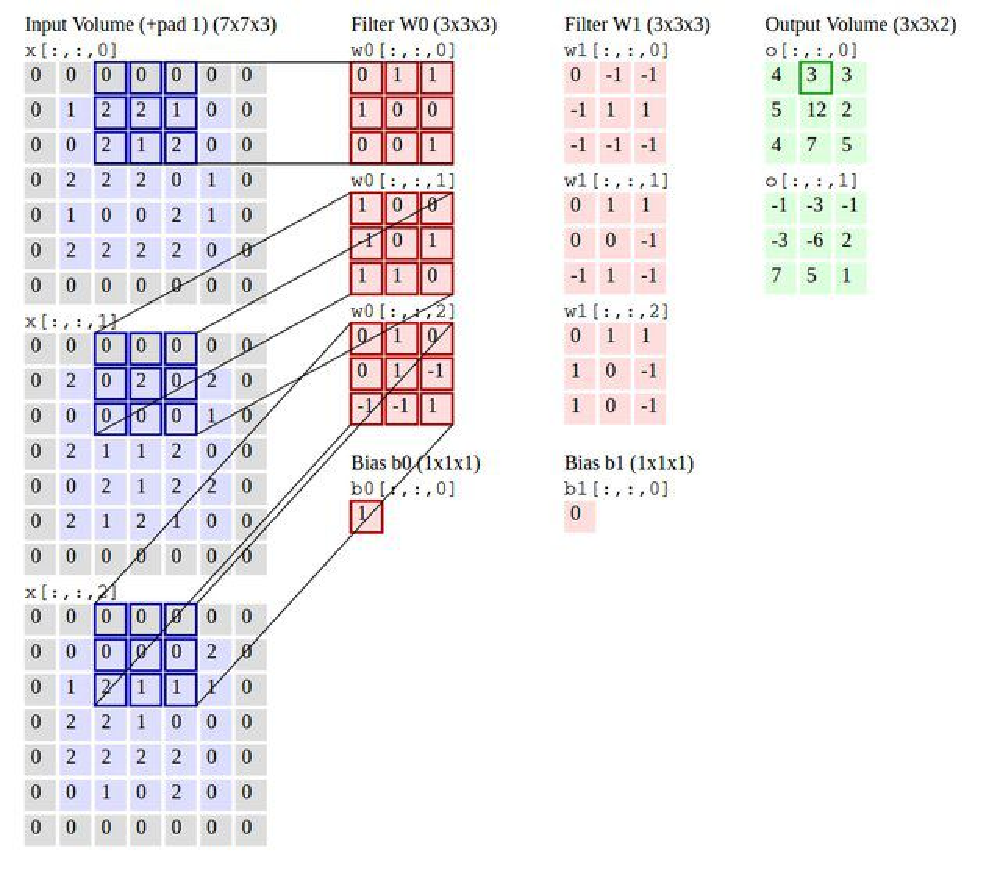
\includegraphics[width=0.7\textwidth]{Convolution_Process.pdf}
\caption{Example of Convolution Process \cite{cnn1}}
\label{fig:convolutionprocess}
\end{figure}

%How to set the convolution kernel can refer to the size and number of the convolution kernel of the convolutional neural network, and 
How to determine the number of convolution layers? Normally we take a small matrix of $(3,3)$. Each value in the convolution kernel is the neuron parameter (i.e. weight) that we need to find (i.e. train). At the beginning, there will be an initial value randomly. When training the network, the network will pass after These parameter values are continuously updated to the propagation until the best parameter value is found. But how do we know which is the ``best'', this is evaluated by a loss function.

The step size of the convolution kernel refers to the movement of the convolution kernel by several grids at a time, with horizontal and vertical directions.

The convolution operation is equivalent to feature extraction, and the convolution kernel is equivalent to a filter to extract the features we need.

%padding
\paragraph{Padding}
After the convolution operation, the dimensions become smaller, and the resulting matrix is smaller than the original matrix, which is difficult to calculate and hard to perform convolution, thus, we need padding. 

Before each convolution operation, we need to wrap a layer of 0 outside the original matrix. It is possible to only fill in horizontally, or only vertically, or 0 on all sides, so that after convolution, the size of output image will be consistent with input image. Figure \ref{fig:padding} below gives an example of padding zeros to an image.

\begin{figure}[h!]
\centering
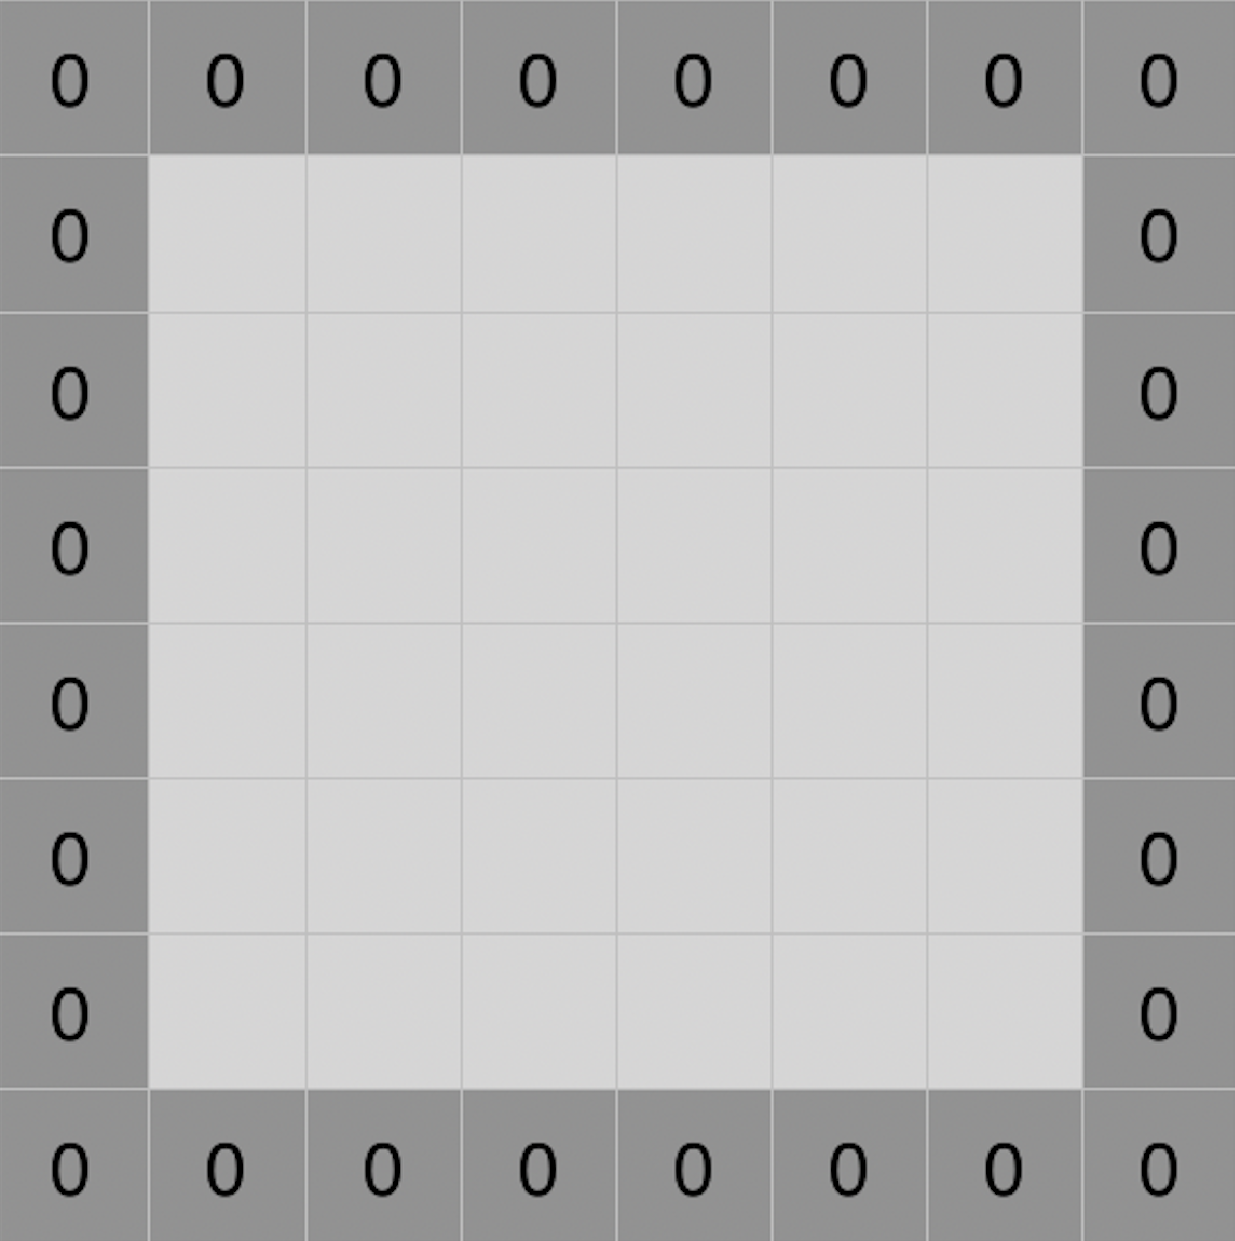
\includegraphics[width=0.2\textwidth]{zeropadding.pdf}
\caption{Example of Zero-padding Added to Image \cite{pooling}}
\label{fig:padding}
\end{figure}

%pooling
\paragraph{Pooling}
After the convolution operation, we extracted a lot of feature information. Adjacent areas have similar feature information and can be replaced with each other. If all these feature information are retained, there will be information redundancy, which increases the computational difficulty. At this time, pooling is equivalent to a dimension reducing operation. 

Pooling happens in a small matrix area. The maximum or average value of the area will be used to replace the area. The size of the small matrix can be set when the network is built. This small matrix is scanning from the upper left corner to the lower right corner when perform pooling.

\begin{figure}[h!]
\centering
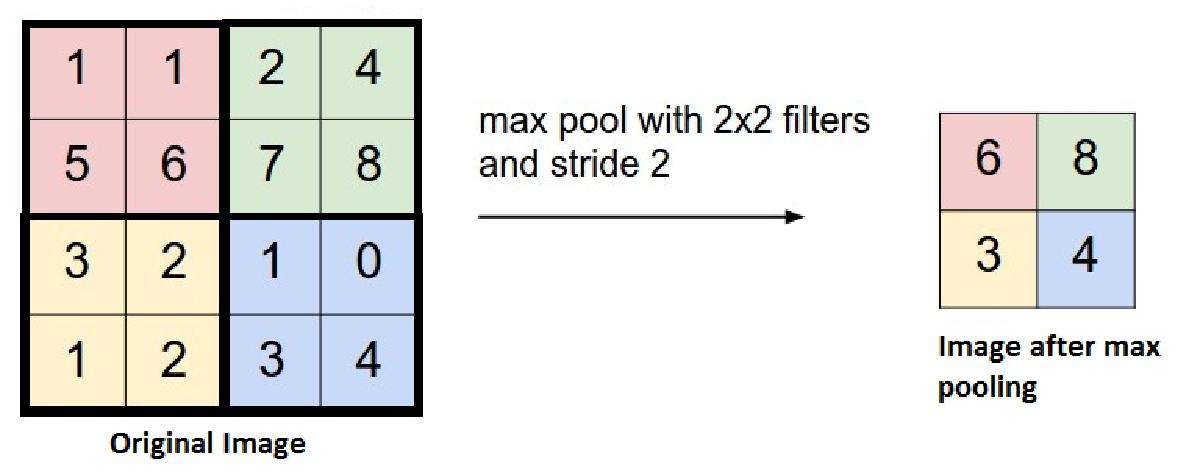
\includegraphics[width=0.65\textwidth]{pooling.pdf}
\caption{Example of Max-pooling \cite{pooling}}
\label{fig:pooling}
\end{figure}

\paragraph{Fully Connected Layer}
%fully connected layers
For layers $n-1$ and $n$, any node in layer $n-1$ is connected to all nodes in layer n. That is, when each node of the $n$-th layer performs calculations, the input of the activation function is the weight of all nodes of the $n-1$ layer. The middle layer like below is fully connected.

\begin{figure}[h!]
\centering
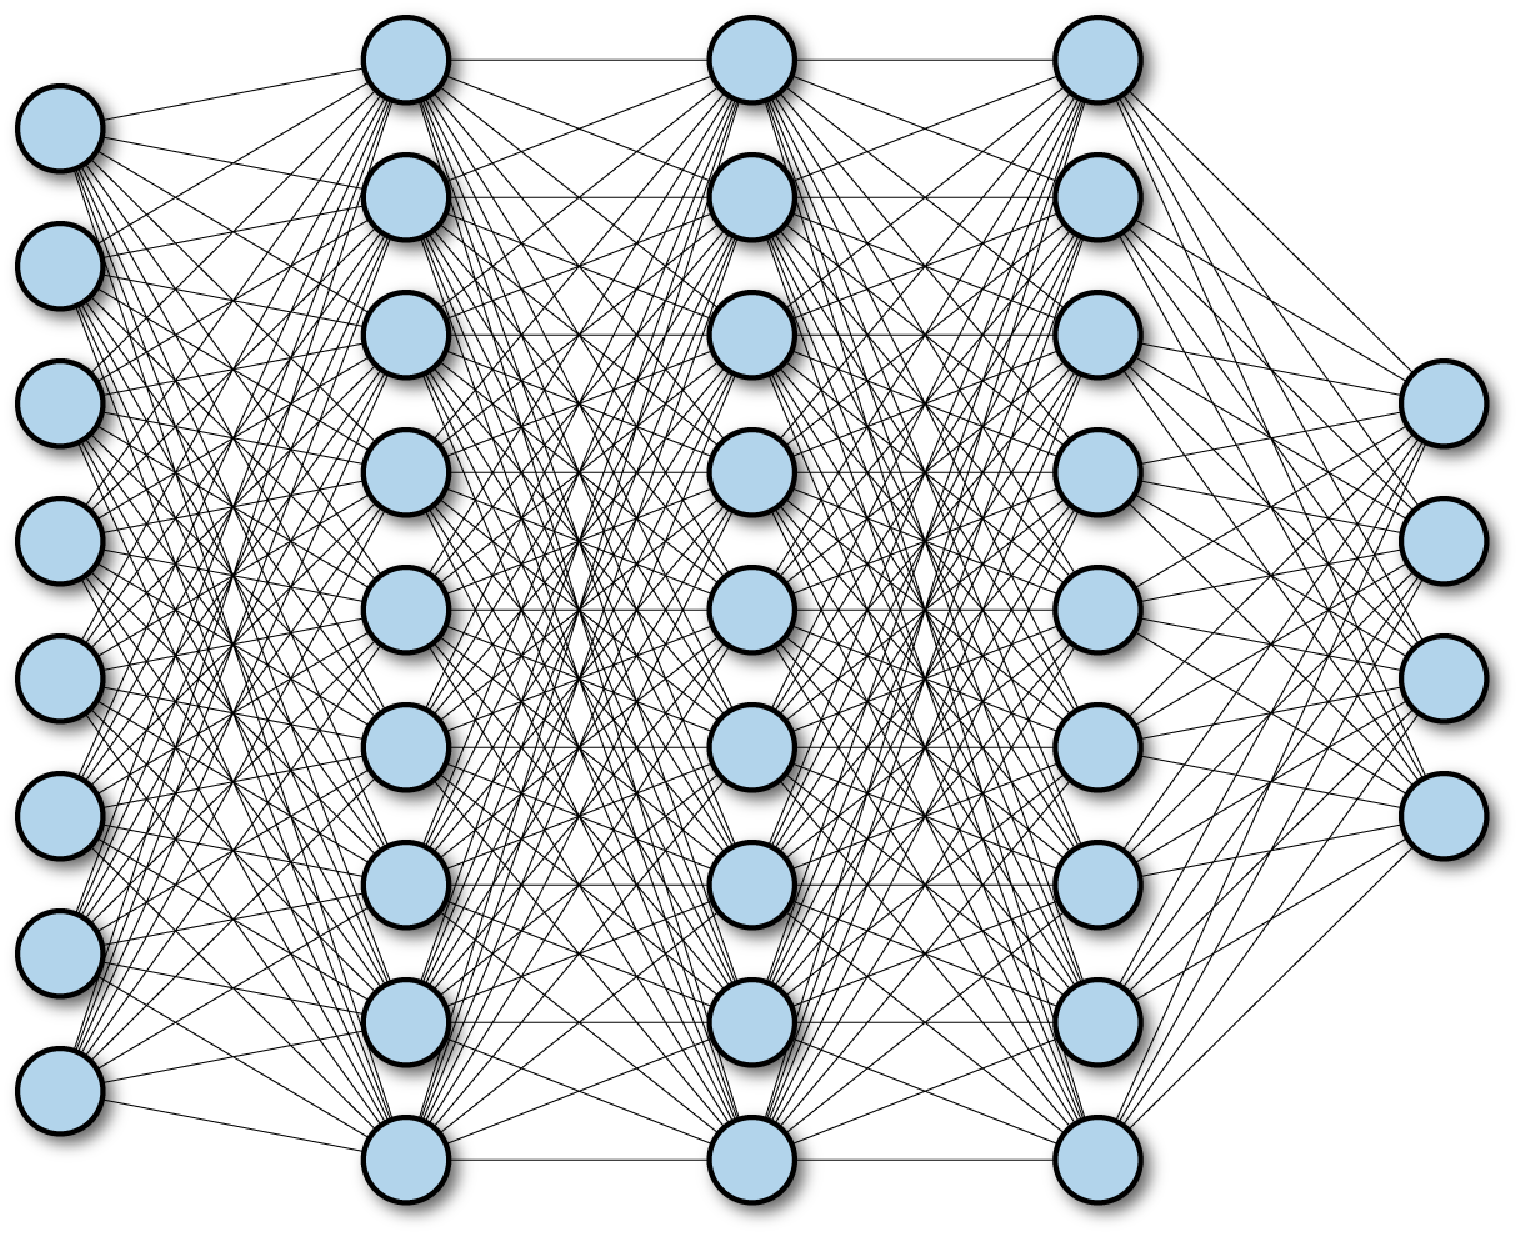
\includegraphics[width=0.5\textwidth]{fullyconnected.pdf}
\caption{Example of Fully Connected Layer}
\label{fig:fully}
\end{figure}

\subsubsection{VGG16}

\verb|VGG16| \cite{vgg16} is a deep network model developed by the computer vision team of Oxford University and researchers at Google DeepMind in 2014. The network has a total of 16 training parameters. The \verb|VGG16| network won the second place in the ILSVRC 2014 competition classification project and the first place in the positioning project, which proved its asset and made it a very commonly used model in the field of CNN.

\paragraph{Configuration}
\verb|VGG| has a relatively simple structure, and its generalisation performance of migrating to other image also achieves well. \verb|VGG| is still often used to extract image features.

According to the different sizes of the convolution kernel and the numbers of convolution layers in VGG, it can be divided into 6 ConvNet configuration: \verb|A|, \verb|A-LRN|, \verb|B|, \verb|C|, \verb|D|, \verb|E|, of which \verb|D| and \verb|E| are more commonly used, which are called \verb|VGG16| and \verb|VGG19| respectively. The following Figure \ref{fig:vgg16config} shows the six structural configurations of VGG. In Figure \ref{fig:vgg16config}, each column corresponds to a structural configuration. For example, section \verb|D| in the figure indicates the structure adopted by \verb|VGG16|.

\begin{figure}[h!]
\centering
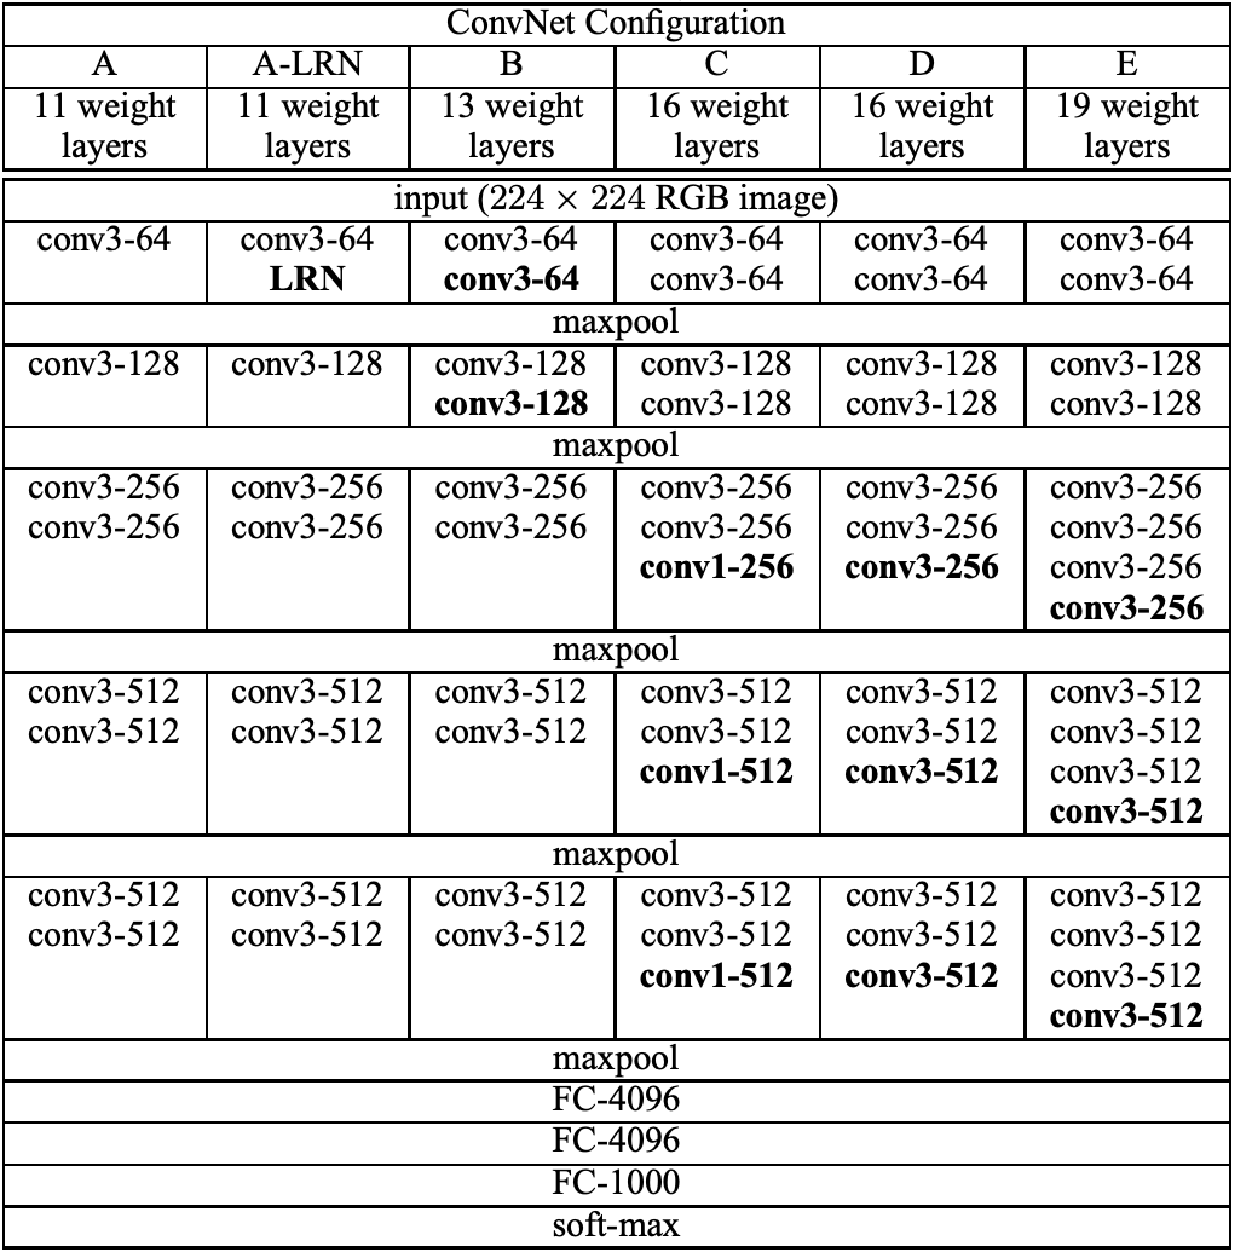
\includegraphics[width=0.7\textwidth]{vgg.pdf}
\caption{ConvNet Configuration of VGG \cite{vgg16}}
\label{fig:vgg16config}
\end{figure}

\verb|VGG16| contains the following components:
\begin{itemize}
    \item 13 Convolutional Layers, each represented by \verb|conv3-XXX|
    \item 3 Fully connected Layers, each represented by \verb|FC-XXXX|
    \item 5 Pool layers, each represented by \verb|maxpool|
\end{itemize}

Among them, the convolutional layer and the fully connected layer have weight coefficients, so they are also called weight layers. The total number is $13+3=16$, which is the source of 16 in \verb|VGG16|. (The pooling layer does not involve weights, so it does not belong to the weighting layer and is not counted).

%features
\paragraph{Structure and Features}
The outstanding feature of \verb|VGG16| is simplicity, which is reflected in:

\begin{itemize}
    \item The convolutional layers all use the same convolution kernel parameters: 
    \item [] The convolution layers are all represented as \verb|conv3-XXX|, where \verb|conv3| indicates that the size of the convolution kernel is 3, that is, the width and height are both 3. And $3\times3$ is very small kernel size, combined with other parameters: \verb|stride = 1|, \verb|padding = same|, so that each convolutional layer (tensor) can maintain the same width and high. \verb|XXX| represents the number of channels of the convolutional layer.
    \item The pooling layer uses the same pooling kernel parameters: 
    \item [] The parameters of the pooling layer are 2 ×
    \item The model is composed of several convolutional layers and pooling layers stacked, which is relatively easy to form a deeper network structure (in 2014, 16 layers have been considered very deep).
    
\end{itemize}

Based on the above analysis, the advantages of \verb|VGG16| can be summarised as: small filters and deeper networks.

Figure \ref{fig:vgg16strucure} illustrates the overall structure of \verb|VGG16|. From left to right, a coloured picture is the input to the network. The white box is the convolution layer, the red is the pooling, the blue is the fully connected layer, and the brown box is the prediction layer. The role of the prediction layer is to convert the information output from the fully connected layer into the corresponding class probability, and play a classification role.

\begin{figure}[h!]
\centering
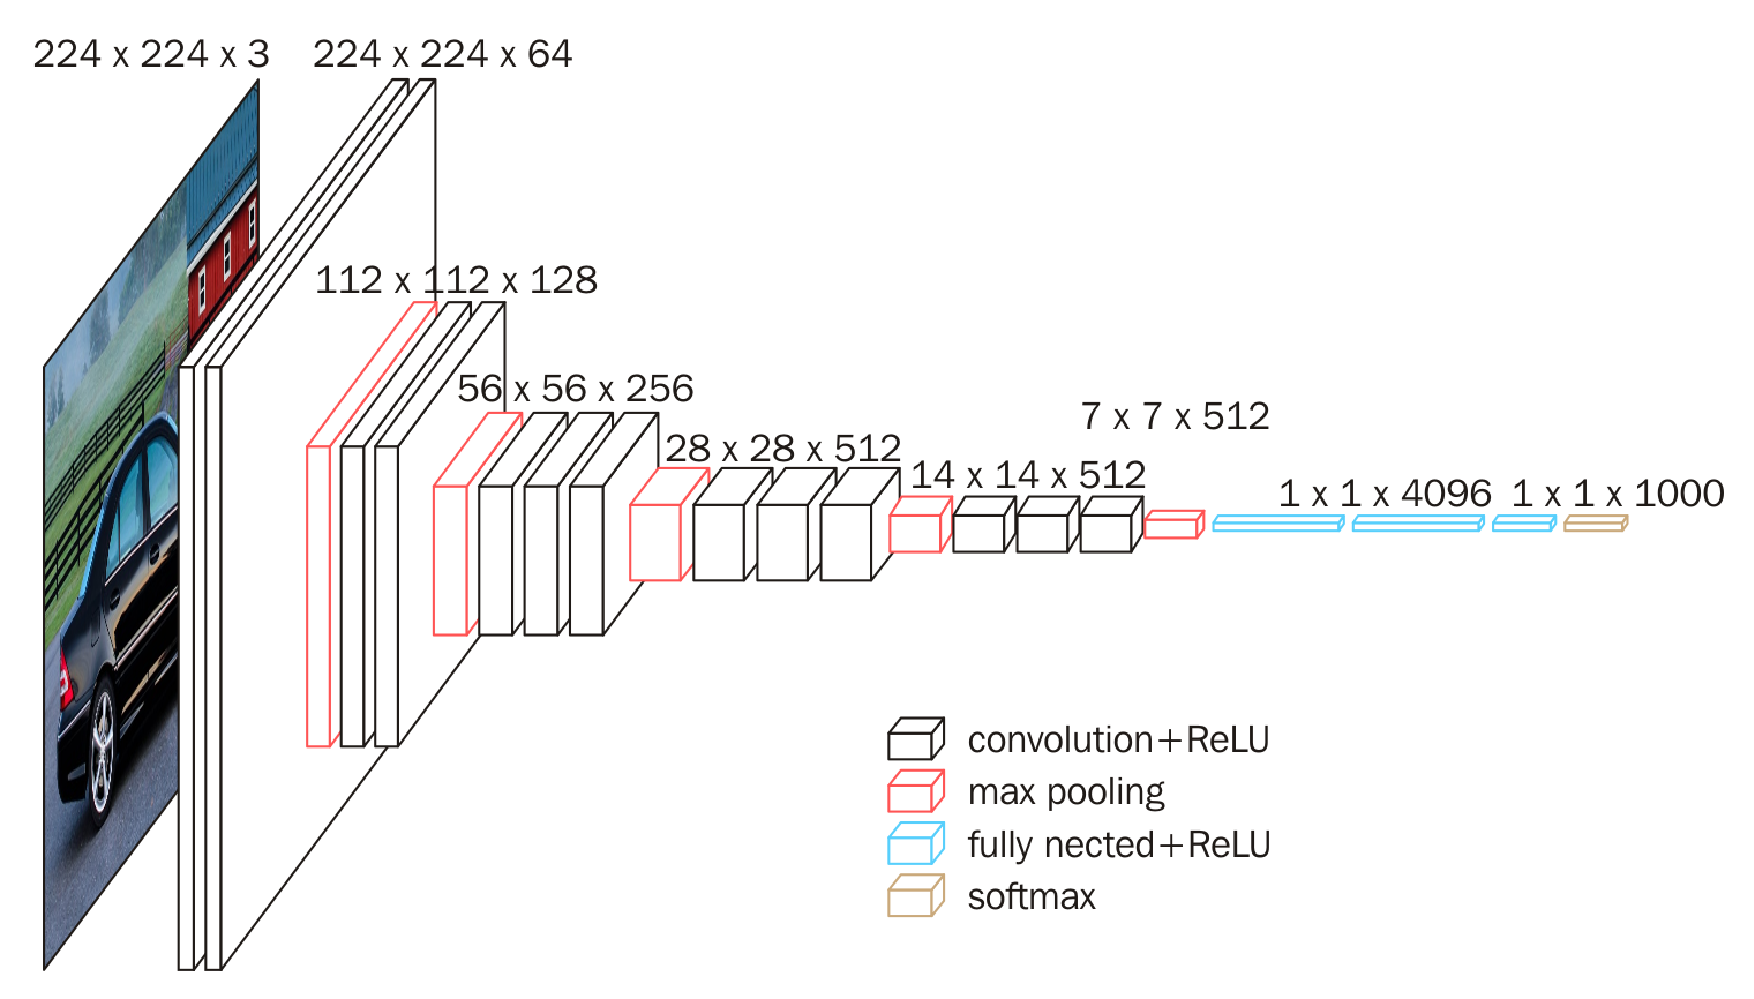
\includegraphics[width=1\textwidth]{vgg16struc.pdf}
\caption{General Structure of VGG16 Model \cite{vgg16}}
\label{fig:vgg16strucure}
\end{figure}

%block structure
\paragraph{Block Structure}
We note that on the right side of Figure \ref{fig:vgg16strucure}, the convolutional layer and pooling layer of \verb|VGG16| can be divided into different blocks, which are numbered \verb|Block1| to \verb|block5| from front to back. Each block contains several convolutional layers and a pooling layer. For example: \verb|Block4| contains:
\begin{itemize}
    \item 3 convolutional layers: \verb|conv3-512|
    \item 1 pooling layer: \verb|maxpool|
\end{itemize}

And in the same block, the number of channels of the convolutional layer is the same, for example:
\begin{itemize}
    \item \verb|block2| contains 2 convolutional layers, each of which is represented by \verb|conv3-128|, that is, the convolution kernel is: $3\times3\times3$, the number of channels is 128
    \item \verb|block3| contains 3 convolution layers, each convolution layer is represented by \verb|conv3-256|, that is, the convolution kernel is: $3\times3\times3$, the number of channels is 256
\end{itemize}

The structure of \verb|VGG16| divided by blocks is given below in Figure \ref{fig:vgg16blockstrucure}.

\begin{figure}[h!]
\centering
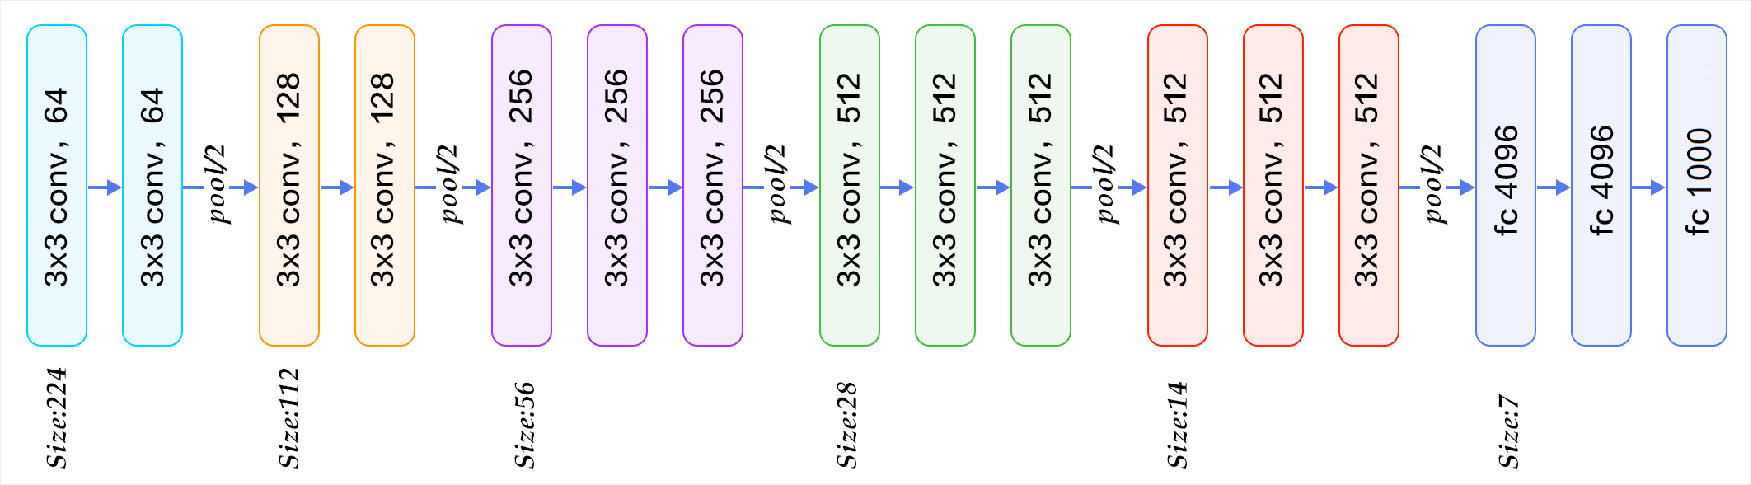
\includegraphics[width=.9\textwidth]{vgg16blockstruc.pdf}
\caption{Structure of VGG16 Model by Blocks \cite{vgg16}}
\label{fig:vgg16blockstrucure}
\end{figure}

The input image of \verb|VGG| is $224\times224\times3$:
\begin{itemize}
    \item The number of channels doubles, from 64 to 128 in order, and then to 256, until 512 remains the same and no longer doubles
    \item Height and width change halved from $224 \to 112 \to 56 \to 28 \to 14 \to 7$
\end{itemize}

\subsubsection{2-stage Model}

The 2-stage model is named for its 2-stage processing of pictures, also known as the region-based method. Here we choose the R-CNN series work as a representative of 2-stage model, which is also the model we adopted for this project.

\subsubsection{R-CNN}
Traditional computer vision methods often use well-designed manual features, such as SIFT and HOG to describe images, while deep learning methods advocate the acquisition of features. From the experience of image classification tasks, the effects obtained by the CNN network automatically acquired features has exceeded the characteristics of manual design. Girshick et al. \cite{rcnn} applied convolutional networks in local areas to give convolutional networks ability to learn high-quality features.

R-CNN abstracts detection into two processes. One is to propose some regions that may contain objects based on the picture, that is, the local cropping of the picture, called the ``Region Proposal''. The paper \cite{rcnn} used the Selective Search algorithm then run the best performing classification network, i.e. AlexNet on the areas, and then obtained the categories of objects in each area. A basic structure of R-CNN is illustrated below as Figure \ref{fig:rcnn}.

\begin{figure}[h!]
\centering
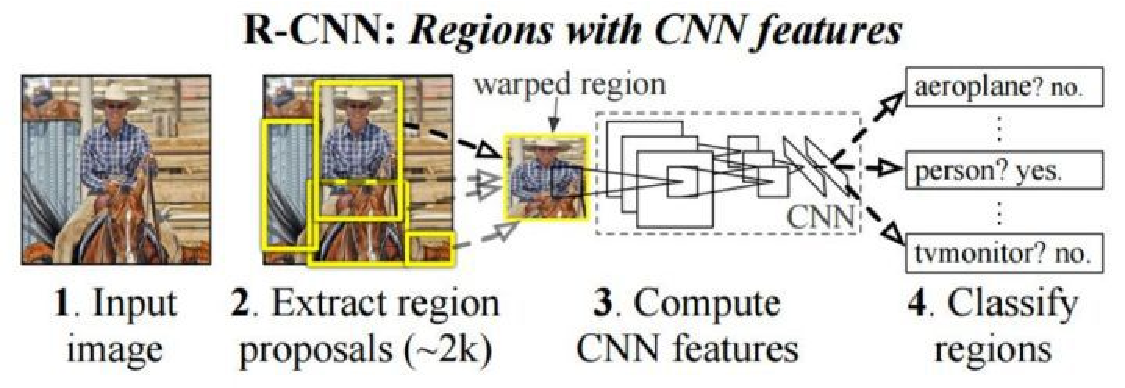
\includegraphics[width=0.7\textwidth]{rcnn.pdf}
\caption{Structure of R-CNN \cite{rcnn}}
\label{fig:rcnn}
\end{figure}

The proposal of R-CNN has two significant contributions: first, CNN can be used for region-based localisation and segmentation of objects; second, when the number of supervised training samples is scarce, pre-trained models on additional data can achieve excellent results after fine-tuning. The first contribution motivated almost all 2-stage methods, and the second contribution used the model trained in the classification task (Imagenet \cite{imagenet}) as the base network. The fine-tuning method for detecting problems has also been used widely in the subsequent works.

The idea of R-CNN is straightforward, the detection task is transformed into a classification task on the region, which is a test of the deep learning method on the detection task. There are also many issues with the model itself, such as the need to train three different models: proposal, classification, regression and performance problems caused by repeated calculations, etc. But R-CNN can still be considered as the pioneer ``the first paper'' in the field.

\subsubsection{Fast R-CNN}
In 2015 Girshick \cite{fastrcnn} pointed out the reason why R-CNN is time-consuming is that CNN is performed separately on each Proposal. Without sharing calculations, it is proposed that after the basic network is run on the entire picture, it is introduced into the R-CNN sub-network, sharing the large Partially calculated, hence the name ``Fast''.

\begin{figure}[h!]
\centering
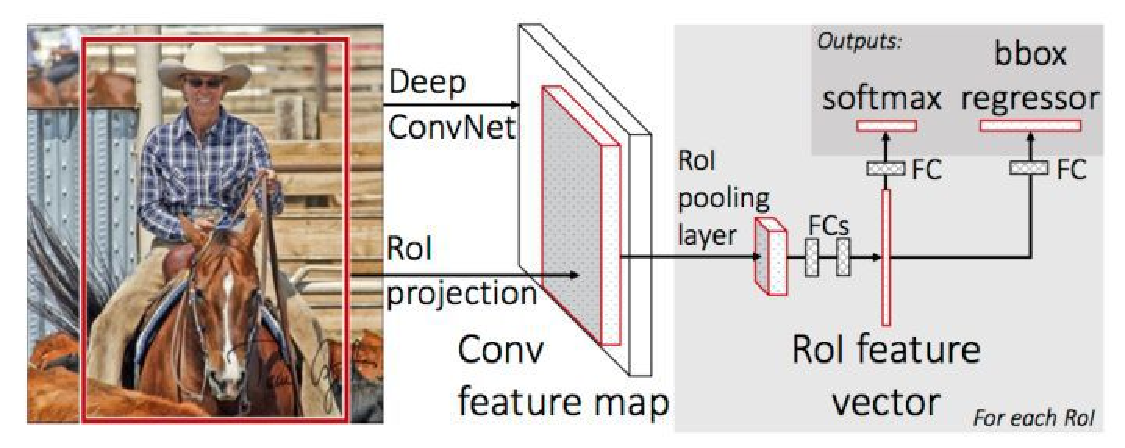
\includegraphics[width=0.7\textwidth]{fastrcnn.pdf}
\caption{Structure of Fast R-CNN \cite{fastrcnn}}
\label{fig:fastrcnn}
\end{figure}

Figure \ref{fig:fastrcnn} above shows the architecture of Fast R-CNN. A feature map is obtained from the feature extractor, at the same time, a Selective Search algorithm is run on the original image and the RoI i.e. Region of Interset, a coordinate group that can be mixed with Region Proposal is mapped to the feature map. Then RoI Pooling is performed for each RoI, this operation obtains feature vectors of equal length, then sorts the obtained feature vectors into positive and negative samples when maintains a certain ratio of positive and negative samples. Next Fast R-CNN batches them into the parallel R-CNN sub-network, performs classification and regression at the same time and unify both losses.

This structure of Fast R-CNN is exactly the prototype of the meta-structure adopted by the mainstream 2-stage method for detection tasks. Fast R-CNN \cite{fastrcnn} unifies Proposal, Feature Extractor, Object Classification and Localisation in a whole structure, and improves the efficiency of feature utilisation through shared convolution calculations, which is the most contributing content.

\subsubsection{Faster R-CNN}
\label{sec:fasterrcnn}
Faster R-CNN \cite{fasterrcnn} is the foundation work of the 2-stage method. The proposed RPN network replaces the Selective Search algorithm so that the detection task can be completed end-to-end by the neural network. Roughly speaking, Faster R-CNN is a combination of RPN plus Fast R-CNN, sharing the characteristics of convolution calculation with RCNN makes the calculation brought by RPN relatively small, so Faster R-CNN can run at 5fps on a single GPU and reaches SOTA in terms of accuracy.

The main contribution of Faster R-CNN \cite{fasterrcnn} is the proposal of Regional Proposal Networks to replace the previous SS algorithm. RPN network models the task of Proposal to the problem of binary classification: whether it is an object. Figure \ref{fig:fasterrcnn} below illustrate the basic structure of Faster R-CNN \cite{fasterrcnn}.

\begin{figure}[h!]
\centering
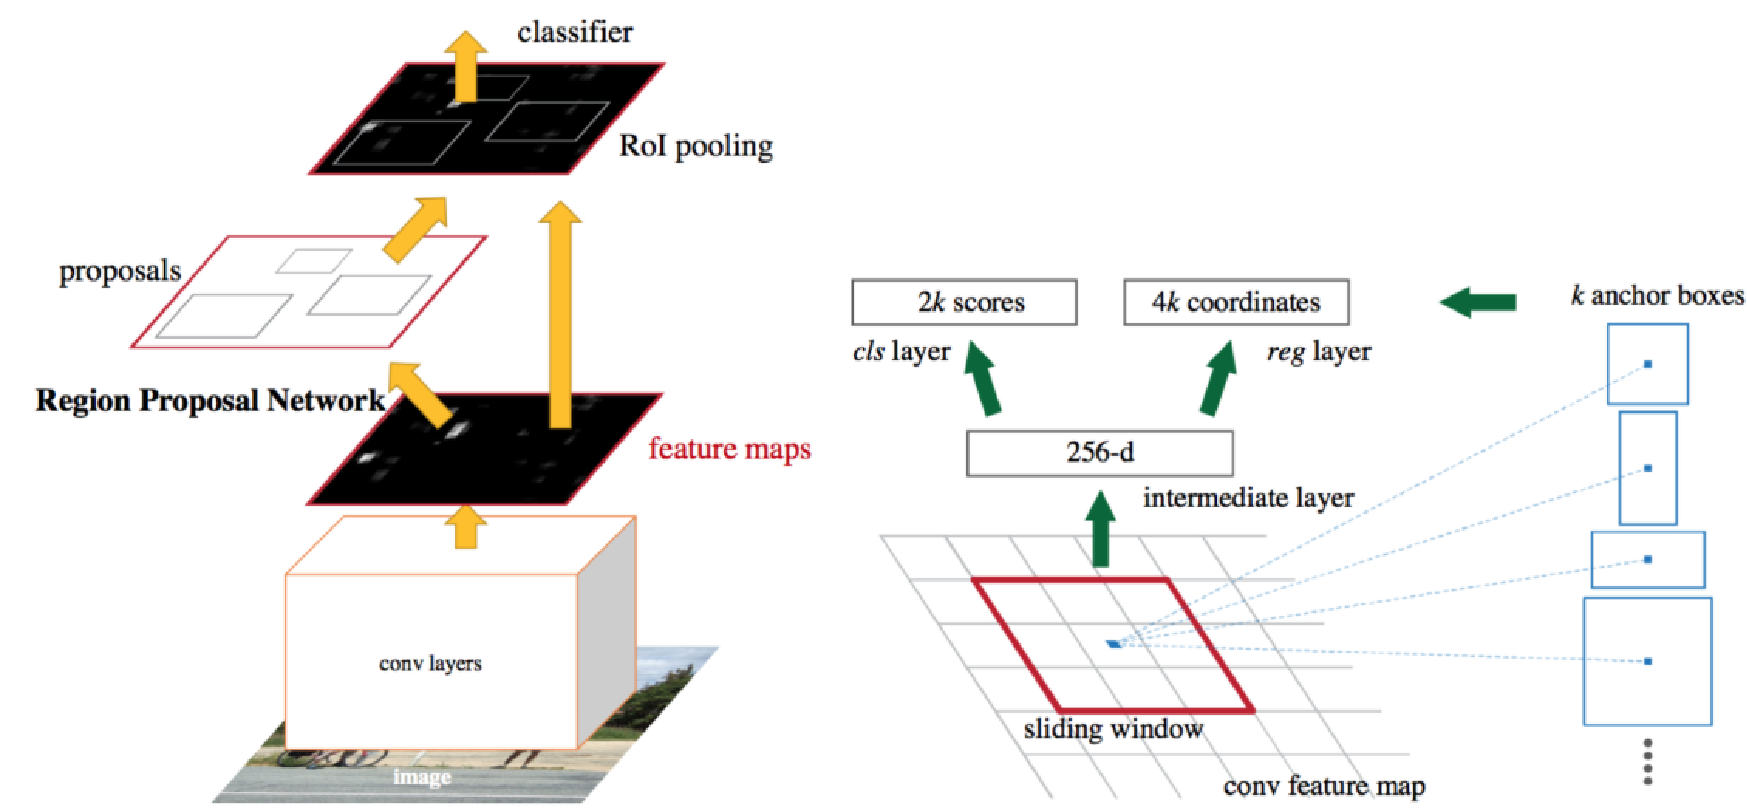
\includegraphics[width=0.8\textwidth]{fasterrcnn.pdf}
\caption{Structure of Faster R-CNN \cite{fasterrcnn}}
\label{fig:fasterrcnn}
\end{figure}

The first step is to generate anchor boxes with various size and aspect ratio on a sliding window (as shown in the right part of Figure \ref{fig:fasterrcnn}), give IoU a predetermined threshold, label anchor box as positive or negative corresponding to the Ground Truth. Thus, the input samples to RPN is organised into anchor box (coordinates) of each anchor box and whether this anchor box has an object or not (binary label). RPN network maps each sample to four coordinate values and a probability value which corresponds the probability of there is an object in the anchor box, values for the four coordinates define the position of the object. Finally, combine the loss of binary and coordinate regression, as the target of training RPN network.

Faster R-CNN completed the ``deep'' part of the inspection tasks using RPN network. The idea of using a sliding window to generate anchor box is also widely adopted such as in YOLO v2, etc. 


\section{Image-text Alignment}
Image-text matching and visual question answering (VQA) are the frontiers of image and text multi modal fusion. The former needs to map images and texts to the same semantic space, and then judge their similarity by distance; the latter needs to find suitable answers in all candidate sets.

\subsection{Convolutional Neural Network Architectures for Matching Natural Language Sentences}

This paper \cite{hu2015convolutional} is a common method for text processing used in Image-Text Matching tasks, which is equivalent to a classic work of natural language processing.

The core idea is to apply the convolution operation to text. The problem to be solved in this article is the matching between Text.

\subsubsection{Text Convolutional}
First of all, we explain the convolution operation of the text. After the discrete text information: embedding is done, the continuous features of the text will be obtained, that is, a word can be represented by a vector. At this time, it is very similar to process an image. A word is equivalent to one pixel in an image, and a sentence is composed of several such words. In a specific implementation, the feature dimension of Embedding can be equivalent to the number of channels in the image, so that the words are connected end to end, and an image with a length of $1\times N$ (the number of text words) is finally formed. At this time, a convolutional network of text can be implemented.

Images can be resized to the same size by linear transformation methods, but text cannot, so the convolution of the text generally uses a Gated Convolutional Layer, that is, for sentences of insufficient length, it is forced to zero, as shown below in Figure \ref{fig:cnnamnls1}:

\begin{figure}[h!]
\centering
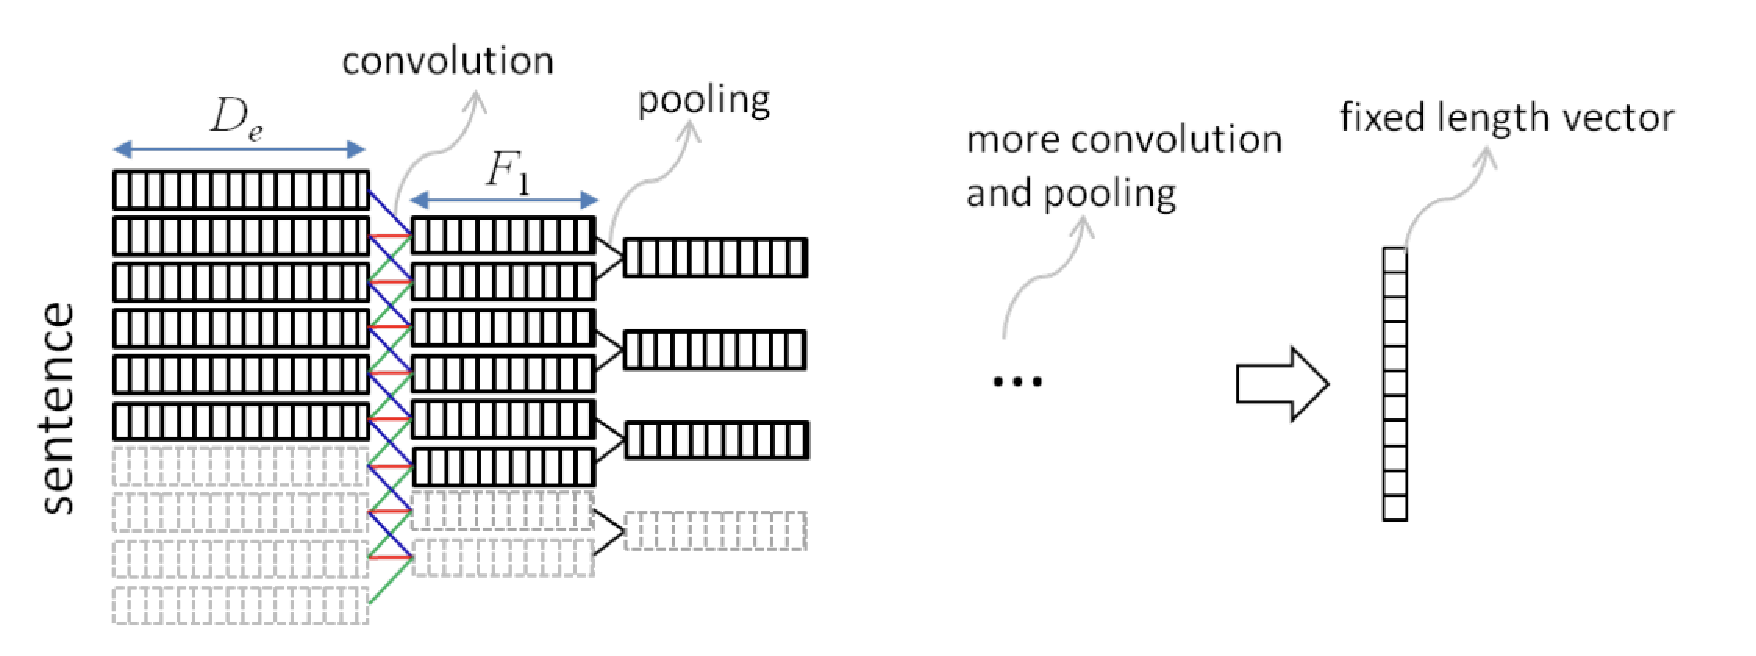
\includegraphics[width=.8\textwidth]{cnnamnls1.pdf}
\caption{Structure of Convolutional Sentence Model \cite{hu2015convolutional}}
\label{fig:cnnamnls1}
\end{figure}

Another point to note is that Maxpooling will be selected as the pooling method for general text so that local features can be maximised accordingly.

\subsubsection{Architecture}
This paper proposed two network structures. One is the matching post-fusion technology, that is, to obtain their vector representation through CNN in two texts to be matched, and then perform stitching and add several layers of full connections to predict the final match.

The network structure of Arc-I is shown in the Figure \ref{fig:cnnamnls2}:

\begin{figure}[h!]
\centering
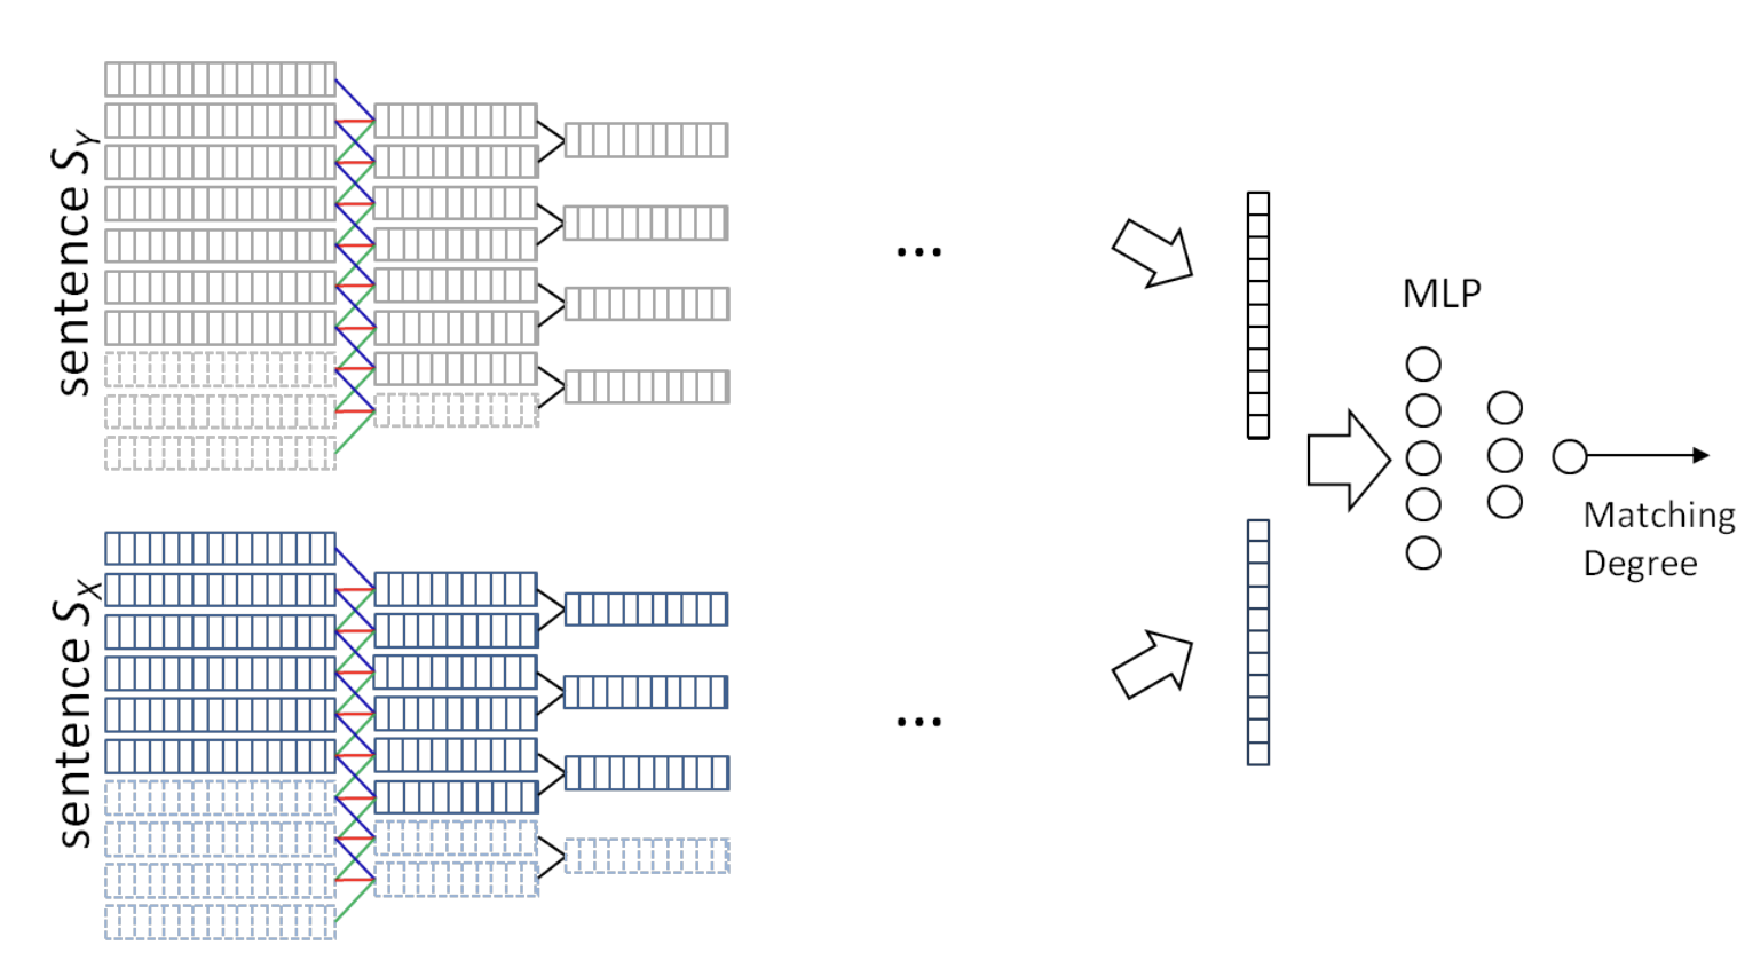
\includegraphics[width=.8\textwidth]{cnnamnls2.pdf}
\caption{Arc-I for matching two sentences \cite{hu2015convolutional}}
\label{fig:cnnamnls2}
\end{figure}

It can be seen from the figure that its feature processing method of encoding belongs to the post-fusion of features, and is very naive. In such a network model, the author did not consider the correlation between different sentences and the order of words, that is, the model mapped the two sentences into a semantic space involuntarily. In order to solve this problem, the author developed a second method:

The network structure of Arc-II is shown in the Figure \ref{fig:cnnamnls3}:

\begin{figure}[h!]
\centering
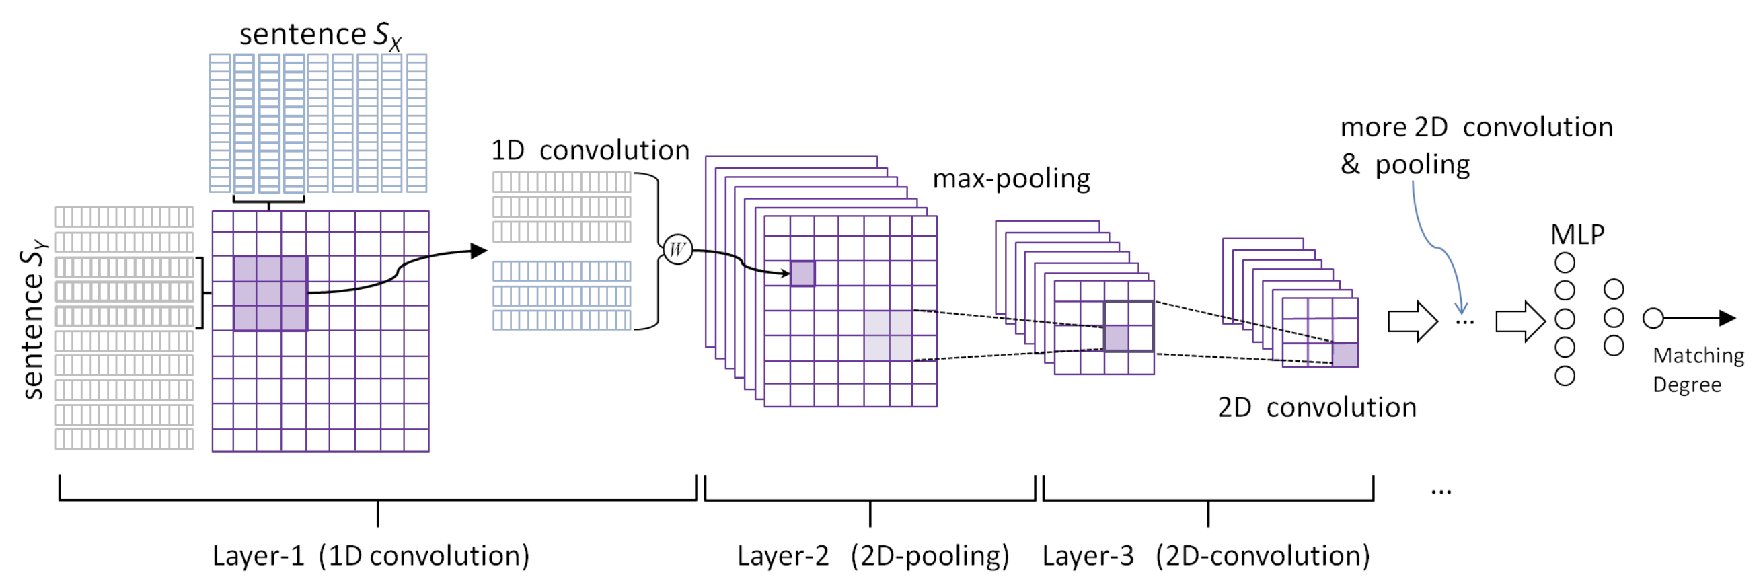
\includegraphics[width=\textwidth]{cnnamnls3.pdf}
\caption{Arc-II of convolutional matching model \cite{hu2015convolutional}}
\label{fig:cnnamnls3}
\end{figure}

This model combined all the word positions of the two sentences, and each position was expressed by the following formula:

$$
\hat{\mathbf{z}}_{i, j}^{(0)}=\left[\mathbf{x}_{i: i+k_{1}-1}^{\top}, \quad \mathbf{y}_{j: j+k_{1}-1}^{\top}\right]^{\top}
$$

$x$ and $y$ respectively represent the sentence to be matched. According to the above formula, the two sentences will form a square \verb|FM1|. Each position of \verb|FM1| is composed of $2k_1$ vectors. That is, this is actually a 4-dimensional structure \verb|[#Sentence * #Sentence * 6 * #Embd_size]|. A one-dimensional convolution using the latter two dimensions will form a three-dimensional feature map of \verb|layer-2|.

Then the network structure behind is the common model in the image.

\subsubsection{Summary}
\begin{itemize}
    \item The convolutional network processes text data and introduces location information into the convolutional network to form a 3d feature map. Gated Convolution, to ensure that the gradient will not be affected when the sentence is not long enough.
    \item MaxPooling guarantees maximum response of local features.
\end{itemize}

\subsection{m-CNNs}

This work \cite{ma2015multimodal} needs to solve the problem of image and text matching. There is not much innovation in image features, that is, features extracted by CNN networks. Different from his previous work, it fuses image features with text features and directly inputs them to the convolutional network for matching. m-CNNs also pays attention to text information with different granularities.

The way m-CNNs deals with features is by directly concatenating the features.

\subsubsection{Word-level Matching CNN}
The finest-grained matching problem. The network structure is as follows:

\begin{figure}[h!]
\centering
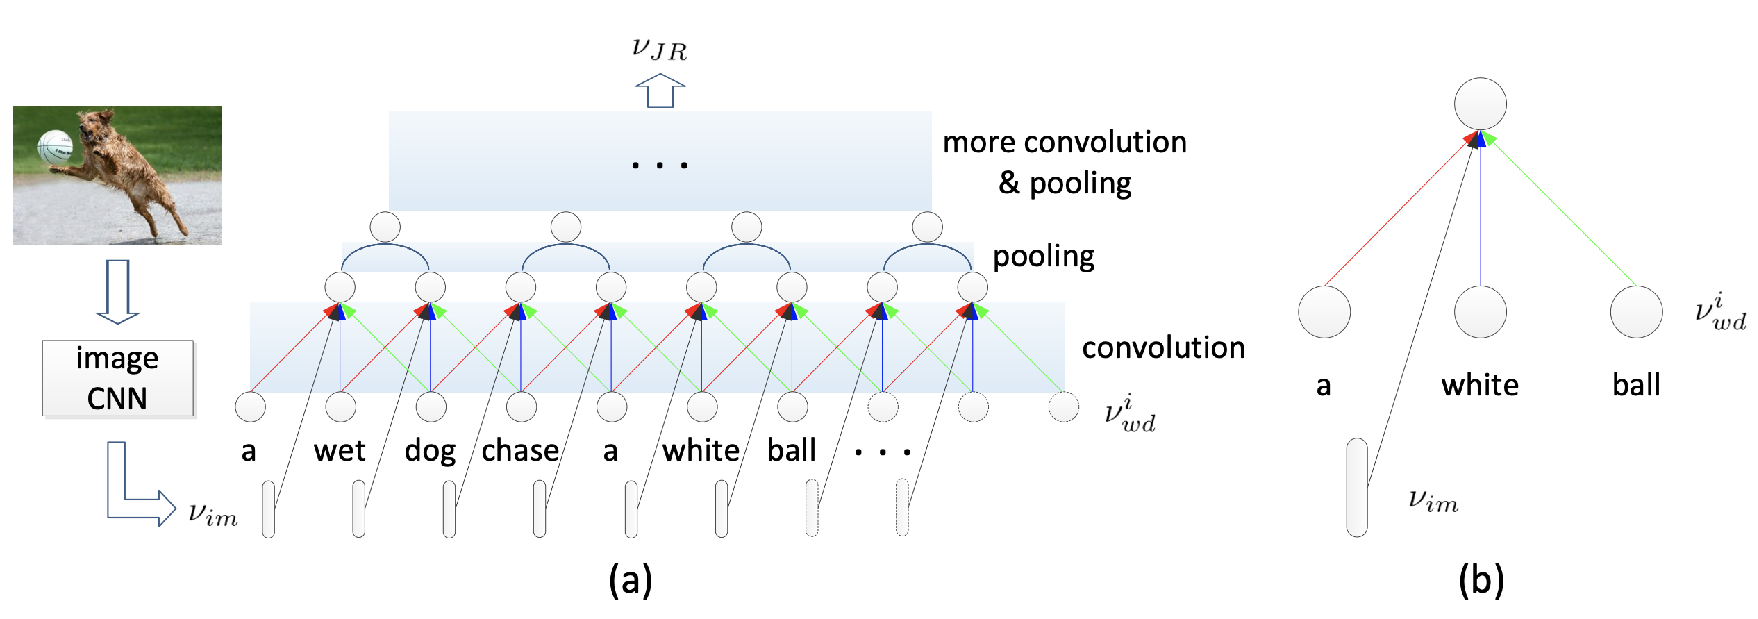
\includegraphics[width=\textwidth]{mccns1.pdf}
\caption{The word-level matching CNN. \cite{ma2015multimodal}}
\label{fig:mccns1}
\end{figure}

The calculation formula is as follows:

$$
\vec{\nu}_{(0)}^{i} \stackrel{\text { def }}{=} \nu_{w d}^{i}\left\|\nu_{w d}^{i+1}\right\| \cdots\left\|\nu_{w d}^{i+k_{r p}-1}\right\| \nu_{i m}
$$

\subsubsection{Phase-level Matching CNN}
Word granularity matching, the network structure is as follows:

\begin{figure}[h!]
\centering
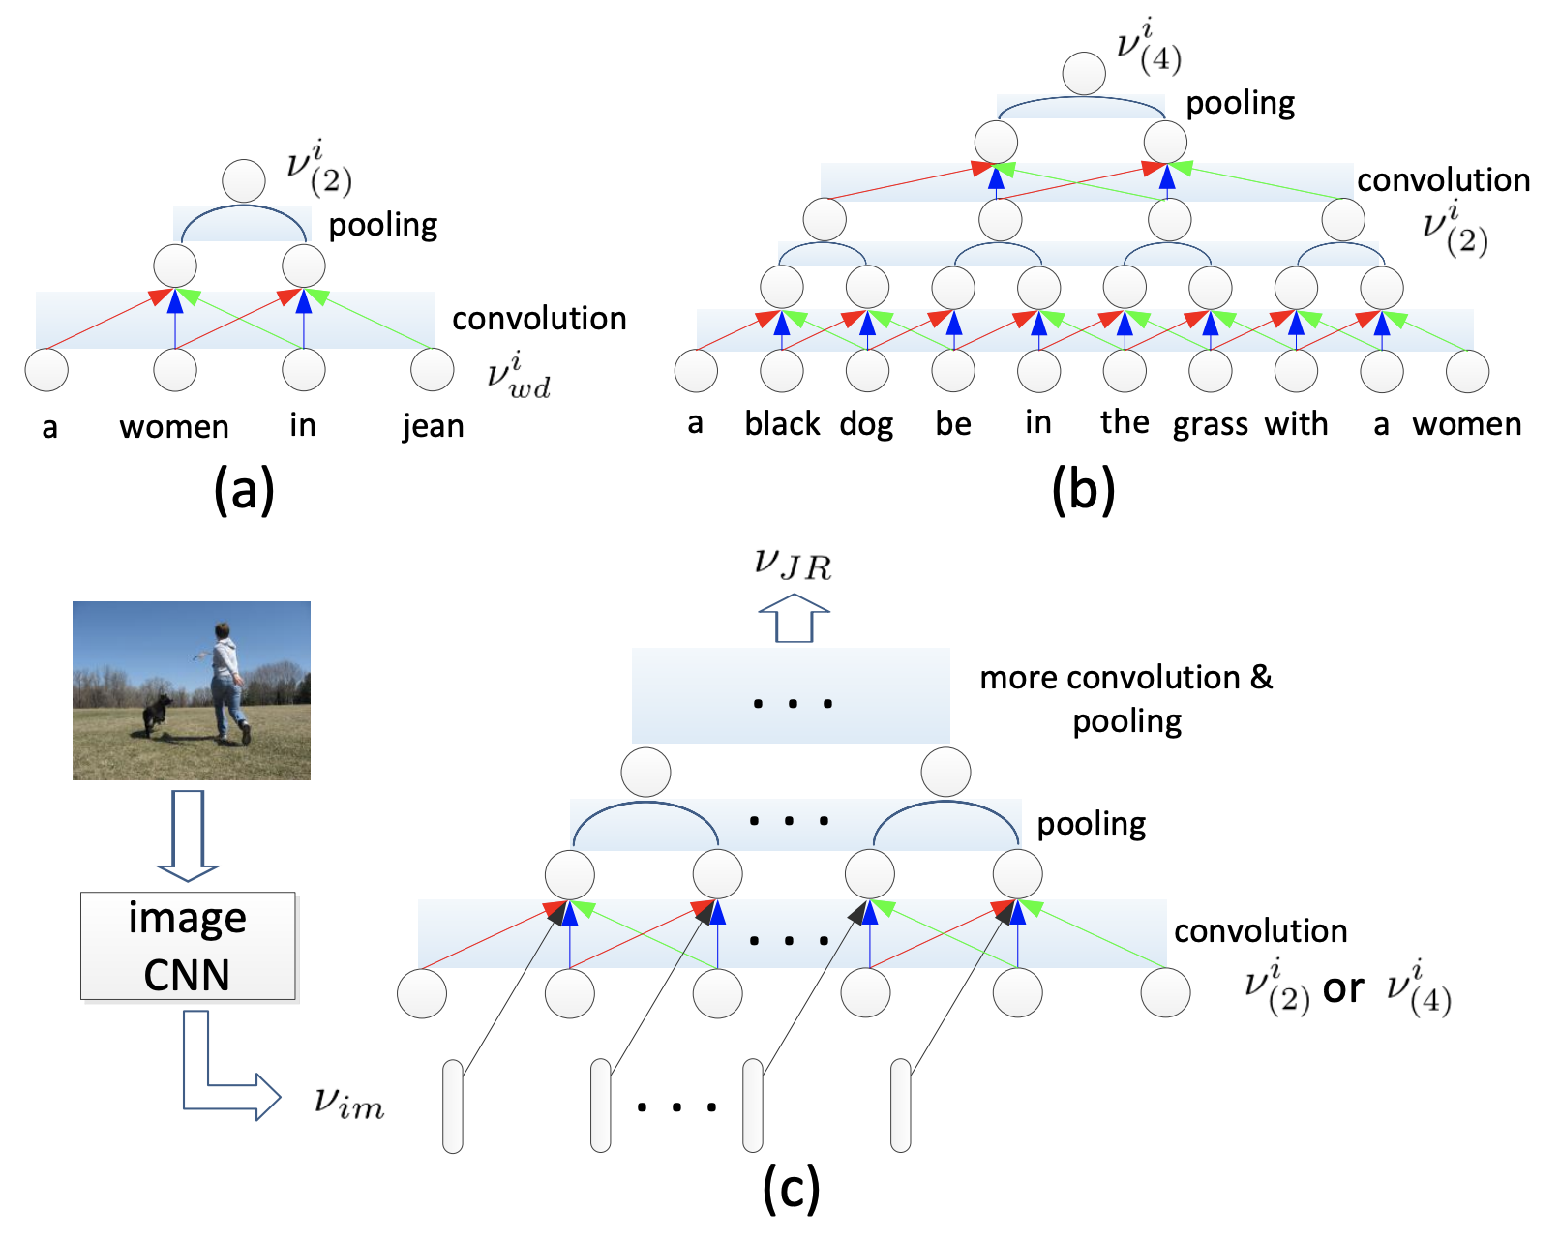
\includegraphics[width=\textwidth]{mccns2.pdf}
\caption{ The phrase-level matching CNN and composed phrases. \cite{ma2015multimodal}}
\label{fig:mccns2}
\end{figure}

The calculation formula is as follows:
$$
\vec{\nu}_{p h}^{i} \stackrel{\text { def }}{=} \nu_{p h}^{i}\left\|\nu_{p h}^{i+1}\right\| \cdots\left\|\nu_{p h}^{i+k_{r p}-1}\right\| \nu_{i m}
$$

Phrase-level matching CNN is similar to word, except that the position is different. The author uses two different granularity phrases in the text, one is two words and one is four words.

A very useful concept in this is the receptive field, which means that a neuron is calculated from a few words. This concept is the same as the concept of the receptive field in an image.

\subsubsection{Sentence-level Matching CNN}
For sentence level matching, the network structure is as follows:

\begin{figure}[h!]
\centering
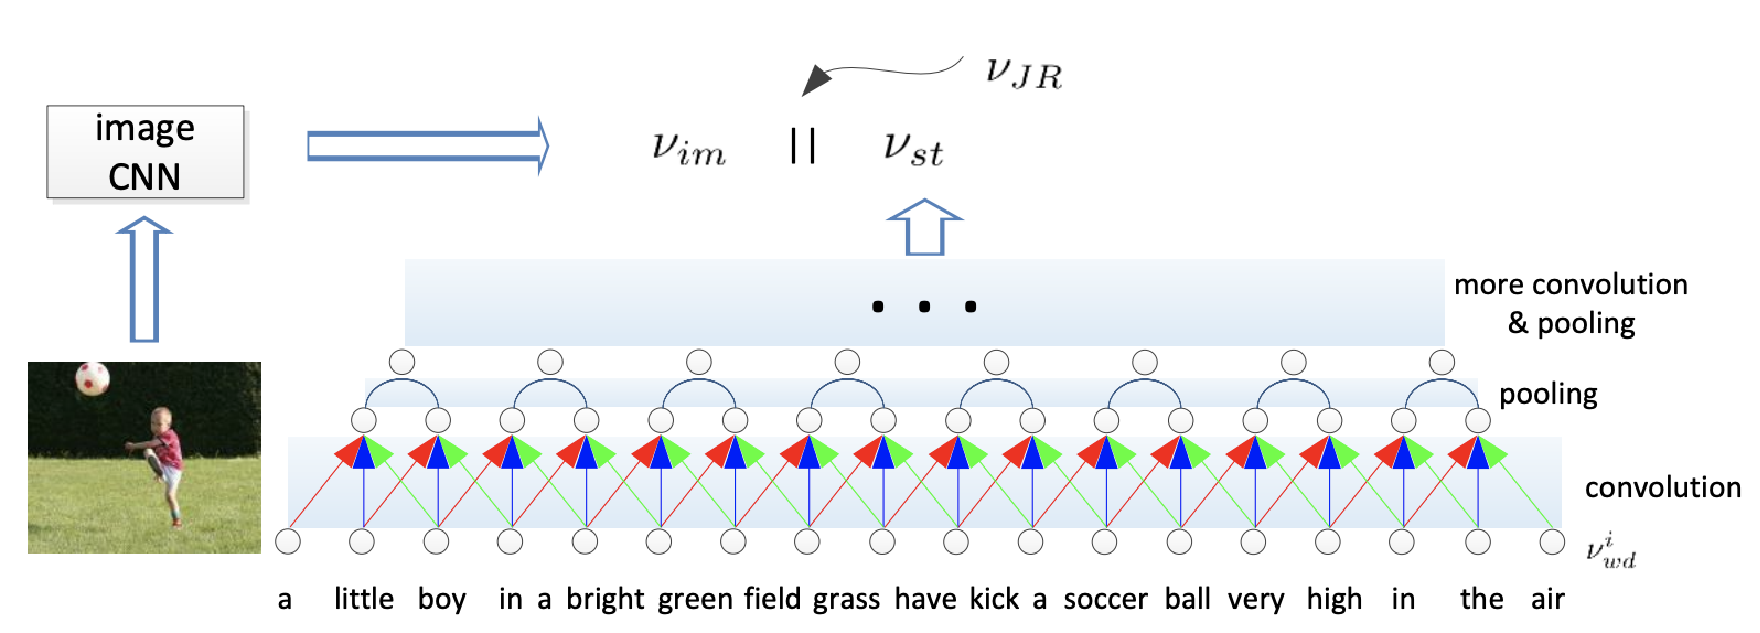
\includegraphics[width=\textwidth]{mcnns3.pdf}
\caption{The sentence-level matching CNN and composed phrases. \cite{ma2015multimodal}}
\label{fig:mccns3}
\end{figure}

Sentence level matching used the last feature for stitching.

From the result, it can be seen that the final ensemble effect is the best, but the performance of the single model is about average.

\subsection{Dual-Path Convolutional Image-Text Embedding}

The problem to be solved in this work \cite{zheng2017dualpath} is also the problem of image and text matching. Unlike the previous two works, it does not use front fusion (generally, the effect of front fusion is better than post fusion). But some interesting ideas were introduced.

\subsubsection{Architecture}
The merit of this network structure is the introduction of residual in text's encoder, which solves the problem of matching images and texts after fusion.

\begin{figure}[h!]
\centering
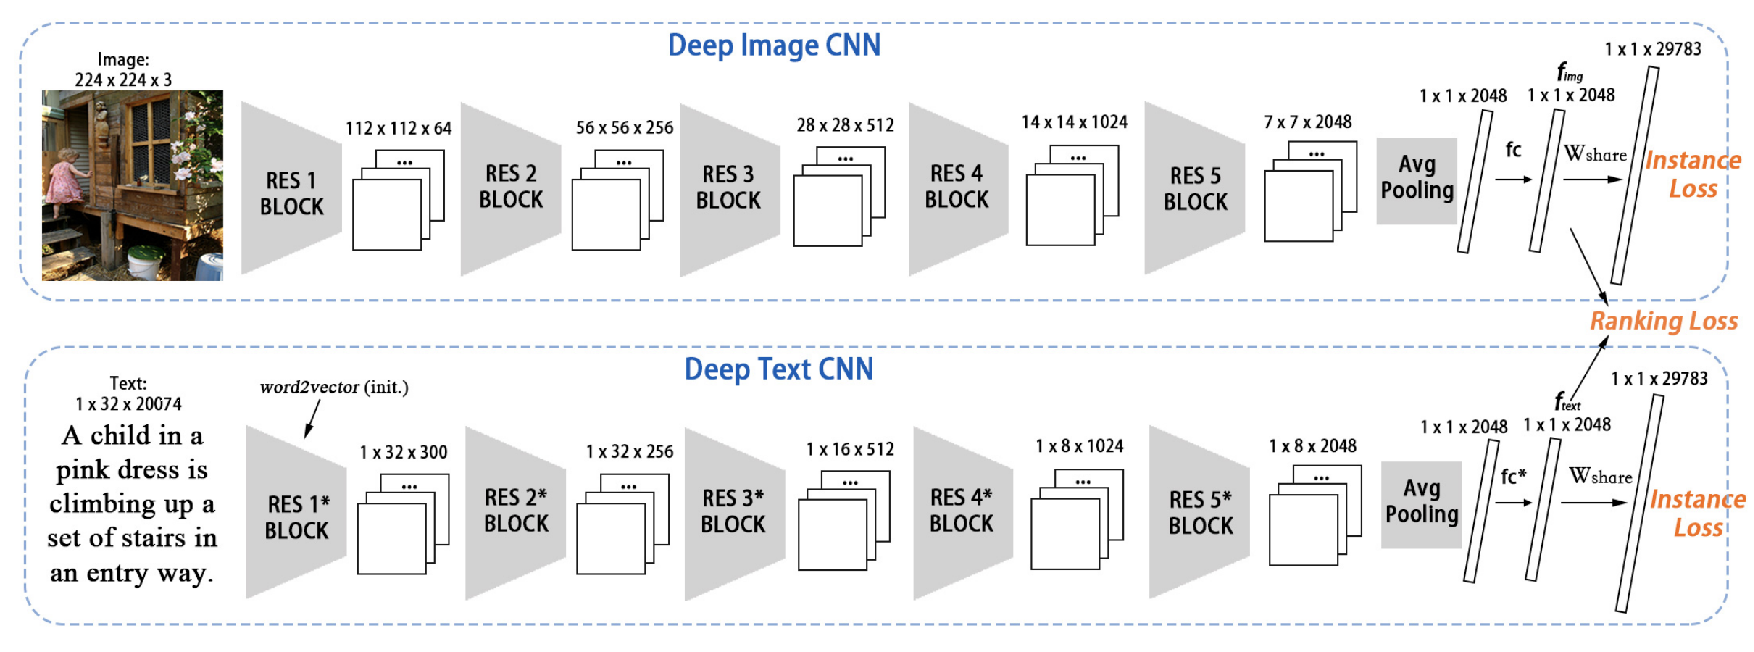
\includegraphics[width=\textwidth]{dpcit1.pdf}
\caption{Architecture of 2 Convolutional Neural Networks \cite{zheng2017dualpath}}
\label{fig:dpcit1}
\end{figure}

\subsubsection{Loss function}
Instance loss was widely discussed in the loss function. The so-called instance loss is the task of doing graphic and text matching. Each pair is used as an instance, and then a \verb|softmax| classifier is used to learn the loss function.

The idea is to adapt the algorithm to the data, that is, to convert the matching problem into a classification problem.

This kind of transformation risk is quite large because our query is diverse; we can never exhaust all query and image pairs, so the basic idea is to achieve it on a multitasking basis.

Before explain multitask loss, we firstly focus on the ranking loss.

The general definition of ranking loss is as follows:

$$
l\left(x_{n}, y_{p o s}, y_{n e g}\right)=\max \left(0, \mu-S\left(x_{n}, y_{p o s}\right)+S\left(x_{n}, y_{n e g}\right)\right)
$$

$S$ is the similarity calculation function, and $\mu$ is the minimum margin in which the similarity needs to be guaranteed. Such ranking loss only considers the loss of $x$ as the matching object, but does not consider $y$. Since $x$ and $y$ are a pair, a two-way loss is required.

Based on this problem, the author proposes the following Ranking loss loss function:

$$
L_{r a n k}=\max \left(0, \alpha-D\left(I_{a}, T_{a}\right)+D\left(I_{a}, T_{n}\right)\right)+\max \left(0, \alpha-D\left(T_{a}, I_{a}\right)+D\left(T_{a}, I_{n}\right)\right)
$$

The front part is Ranking Loss of Image, and the back part is Ranking Loss of Text.

So the final author's loss consists of a total of 3 parts, namely Ranking loss, visual Instance loss, and text Instance loss.

$$
L=\lambda_{1} L_{r a n k}+\lambda_{2} L_{v i s u a l}+\lambda_{3} L_{t e x t u a l}
$$

where $\lambda_{1}, \lambda_{2}, \lambda_{3}$ are predefined weights for different losses.

\subsubsection{Some Interesting Tricks}
This work contains many interesting tricks to achieve better results which we will point out as follows.

\begin{enumerate}
    \item Embedding models initialised with \verb|word2vec| are better than random initialisation.
    \item Sentence jittering, the model randomly adds a certain amount of zero padding to the beginning and end of the sentence.
    \item Instance loss finally shares a same weight parameter to ensure that the information of two different modalities is mapped to the same space.
\end{enumerate}

Two stage training is also the highlight of this article:

\begin{itemize}
    \item Stage-I. At this stage, text residual network is firstly trained. Then it fixes the ranking loss and image in CNN models, so that the CNN of text can be trained. The reason of doing this is the network of text was randomly initialised. To add ranking loss because the image and text are definitely not in the same semantic space at the beginning, we are worried that this loss will be brought into the network of text. Fixing the image CNN because we do not want the gradient of the image and the gradient of the text to interfere with each other.
    
    \item Stage-II, when text's CNN training converges, adding ranking loss and image CNN to the model, and training end-to-end together, the final result is the best.
\end{itemize}

\subsection{DANs}

The main research contribution of DAN \cite{dan} is to introduce attention mechanism into neural network model. The starting point is relatively obvious: the ultimate problem of image and text matching is the matching problem between the entire text and the entire Image, however, this problem is more challenging to solve, so a basic solution is to split the tasks. Text is composed of different words, while image is composed of different regions. If we can match the words of text to the regions of image, this problem will become simpler.

The basic idea is to use the attention mechanism to match text words with image regions in the network automatically. The author cites two types of attention mechanisms: visual attention and text attention.

Both types of attention used the previous state and determine the ``position'' of attention for the next state.

\subsubsection{Visual Attention}
The formula for visual attention is:

$$
\mathbf{h}_{\mathbf{v}, n}^{(k)} =\tanh \left(\mathbf{W}_{\mathbf{v}}^{(k)} \mathbf{v}_{n}\right) \odot \tanh \left(\mathbf{W}_{\mathbf{v}, \mathbf{m}}^{(k)} \mathbf{m}_{\mathbf{v}}^{(k-1)}\right)
$$
$$
\alpha_{\mathbf{v}, n}^{(k)} =\operatorname{softmax}\left(\mathbf{W}_{\mathbf{v}, \mathbf{h}}^{(k)} \mathbf{h}_{\mathbf{v}, n}^{(k)}\right)
$$
$$
\mathbf{v}^{(k)} &=\tanh \left(\mathbf{P}^{(k)} \sum_{n=1}^{N} \alpha_{\mathbf{v}, n}^{(k)} \mathbf{v}_{n}\right)
$$


All $\mathbf{W}$ in the formula are parameters that the network needs to learn, $\mathbf{h}$ is the hidden state, and $\mathbf{m}$ is the memory vector.

\subsubsection{Textual Attention}
The formula for textual attention is:

$$
\mathbf{h}_{\mathbf{u}, t}^{(k)} =\tanh \left(\mathbf{W}_{\mathbf{u}}^{(k)} \mathbf{u}_{t}\right) \odot \tanh \left(\mathbf{W}_{\mathbf{u}, \mathbf{m}}^{(k)} \mathbf{m}_{\mathbf{u}}^{(k-1)}\right)
$$
$$
\alpha_{\mathbf{u}, t}^{(k)}=\operatorname{softmax}\left(\mathbf{W}_{\mathbf{u}, \mathbf{h}}^{(k)} \mathbf{h}_{\mathbf{u}, t}^{(k)}\right)
$$
$$
\mathbf{u}^{(k)}=\sum_{t} \alpha_{\mathbf{u}, t}^{(k)} \mathbf{u}_{t}
$$

The step size $\mathbf{K}$ of the two Attentions is a super parameter, and the author proves that $\mathbf{K}=2$ is the best in experiments.

\subsubsection{Visual and Textual Representation}

The visual features use the features of the second layer of Resnet or VGG, and the text features use the features of bidirectional RNN (LSTM). The visual features are shown in the following Figure \ref{dan1}:

\begin{figure}[h!]
\centering
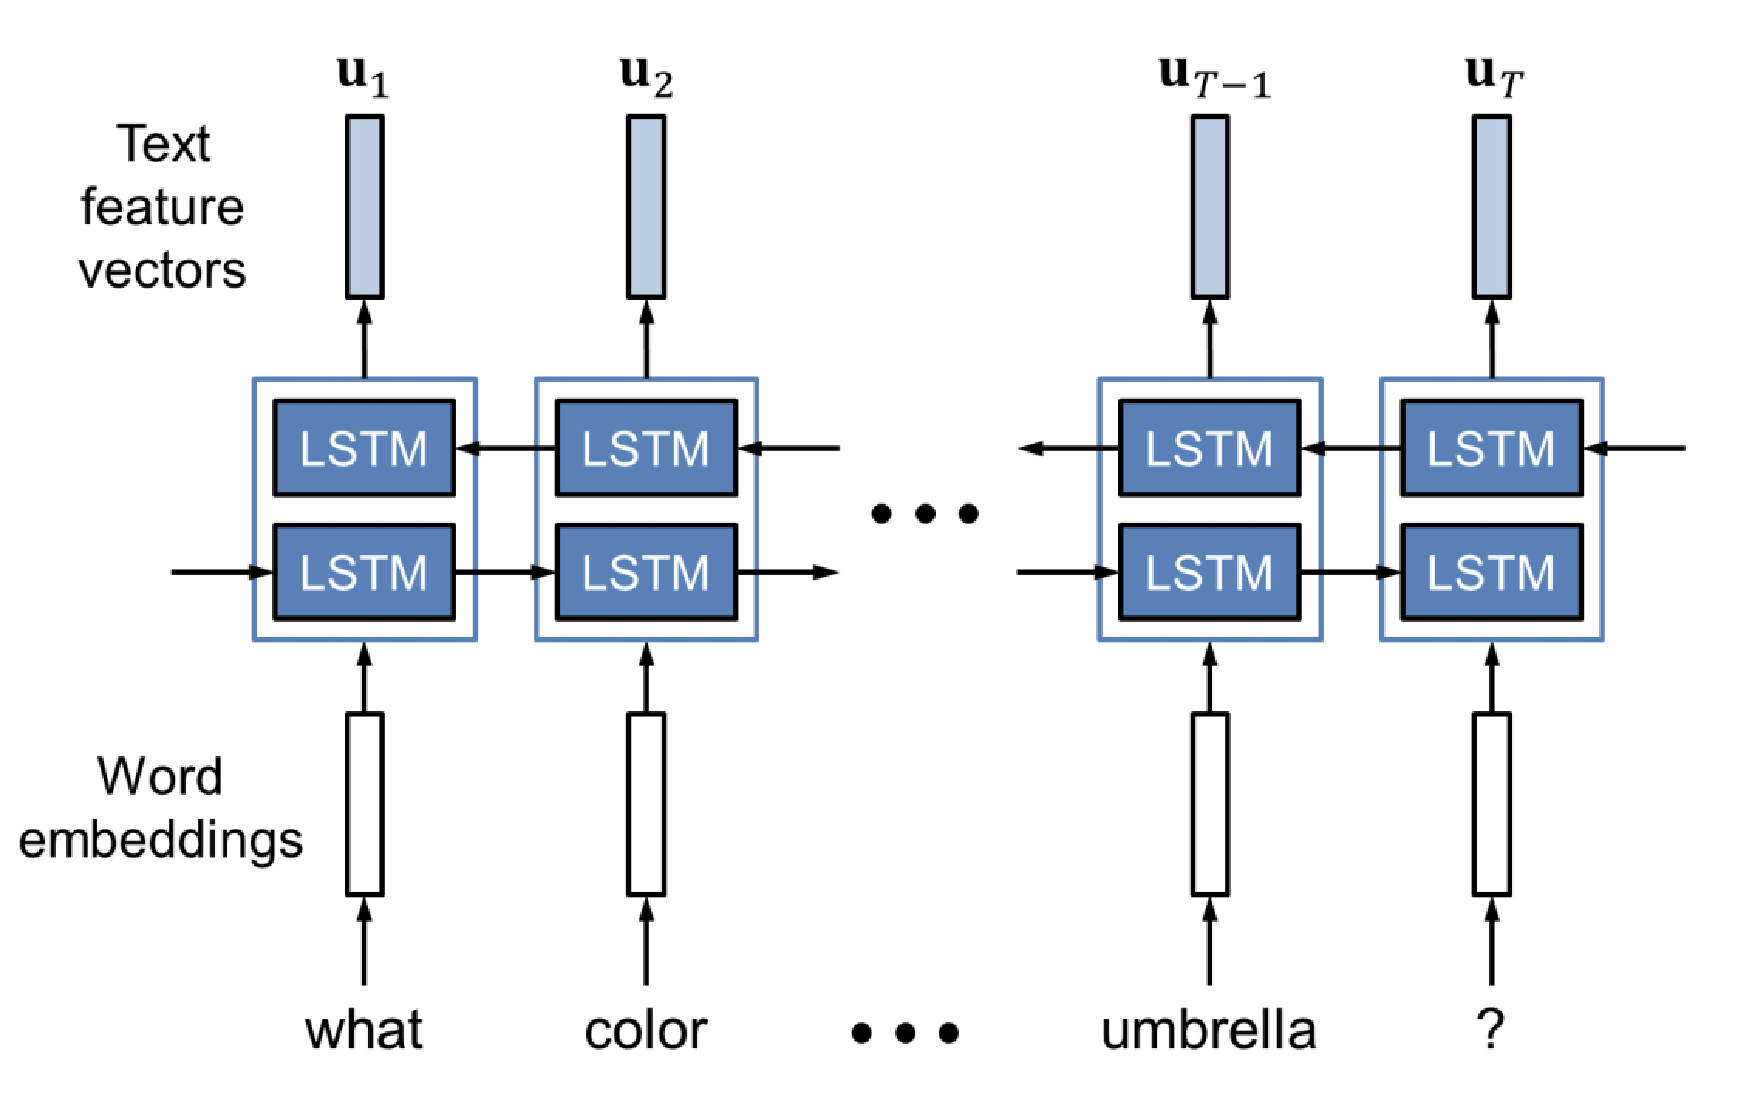
\includegraphics[width=0.8\textwidth]{dans1.pdf}
\caption{Bidirectional LSTMs for text encoding \cite{dan}}
\label{fig:dan1}
\end{figure}

\subsubsection{VQA and Image-Text Matching}

This research solved two different problems which both used the previous attention mechanism. However, the methods of applying attention are different.

\paragraph{Visual Question and Answer}

In the VQA dataset, all the answers are one single word, so in essence, this problem is a classification problem, that is, we need to know which one of the answer sets the question is in the end.

The network structure diagram is displayed as follows in Figure \ref{fig:dan2}:

\begin{figure}[h!]
\centering
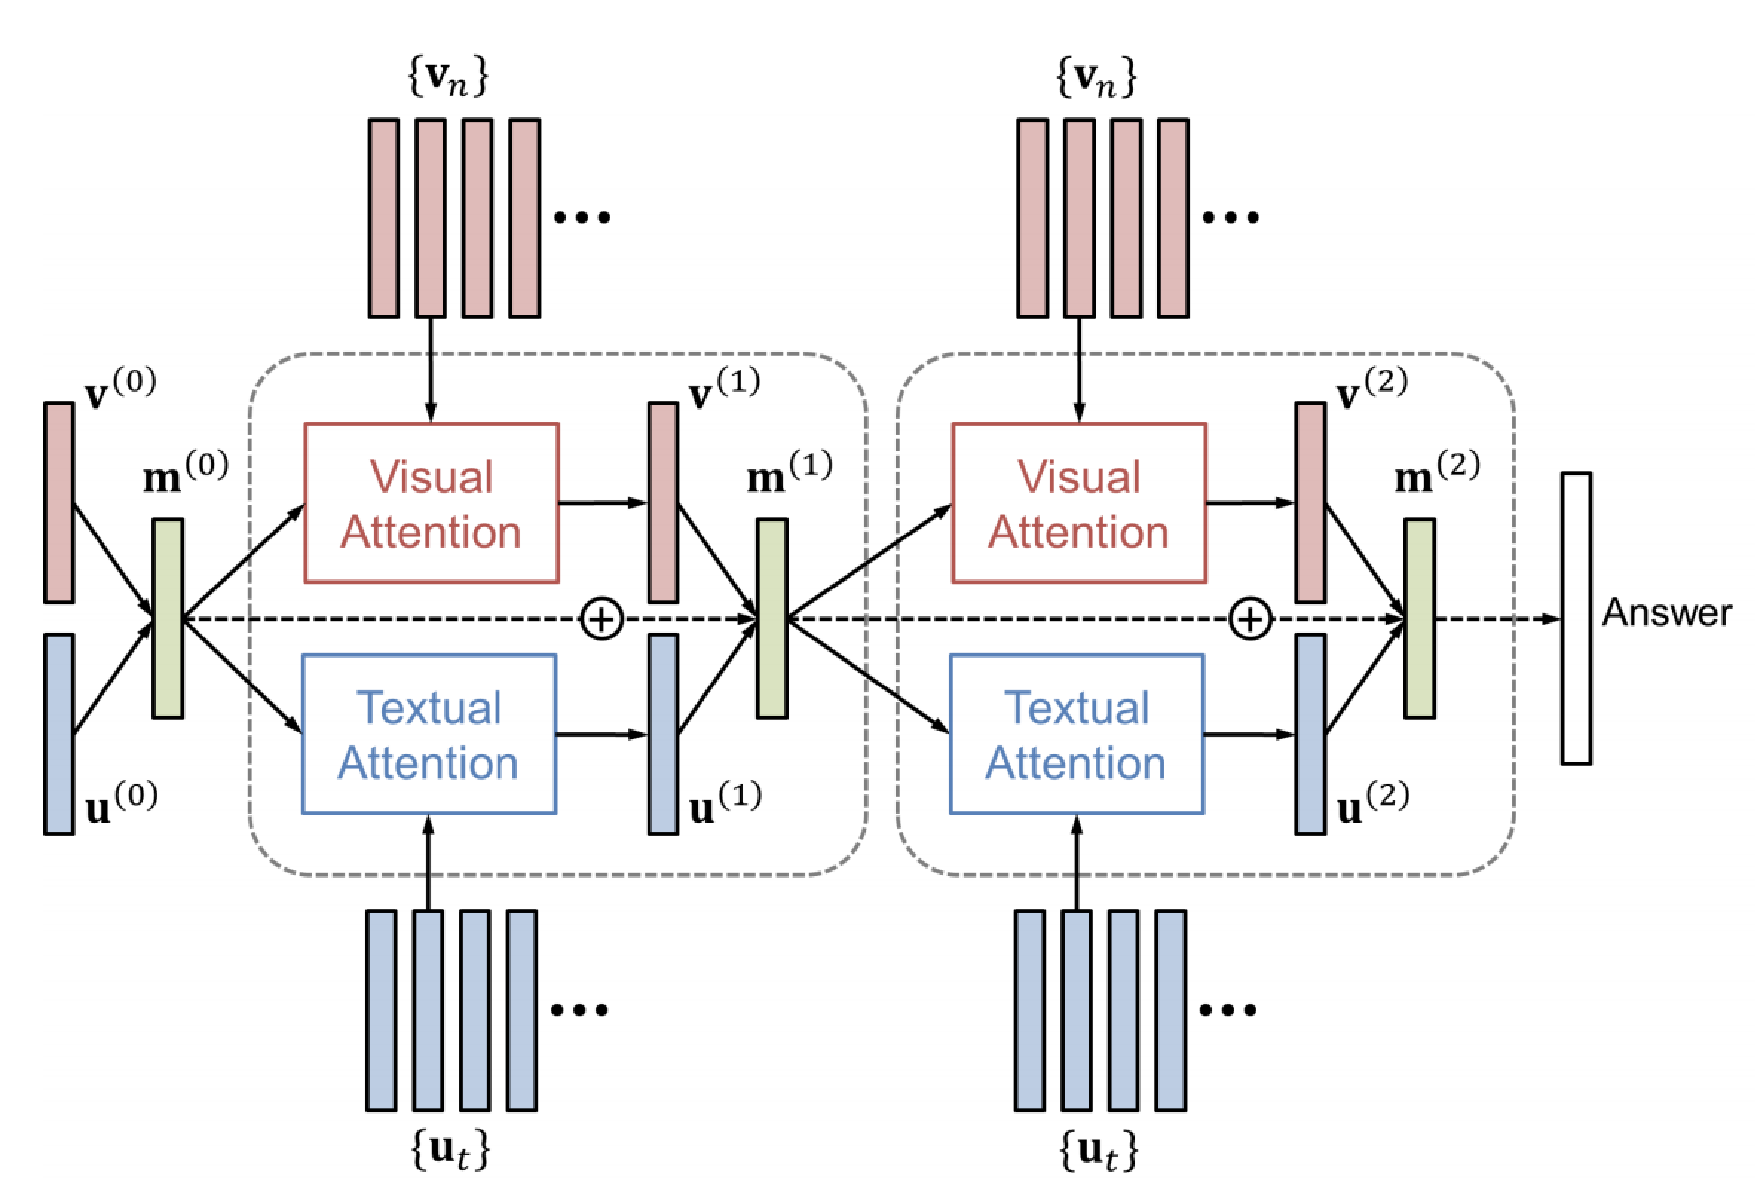
\includegraphics[width=0.8\textwidth]{dan2.pdf}
\caption{r-DAN in case of $\mathbf{K}=2$ \cite{dan}}
\label{fig:dan2}
\end{figure}

As can be seen from the figure, it uses the last memory vector for classification.

The memory vector calculation formula is as follows:

$$
\mathbf{m}^{(k)}=\mathbf{m}^{(k-1)}+\mathbf{v}^{(k)} \odot \mathbf{u}^{(k)}
$$

The initialisation of different parameters is as follows:

$$
\mathbf{m}^{(0)}=\mathbf{v}^{(0)} \odot \mathbf{u}^{(0)}
$$
where
$$
\mathbf{v}^{(0)}=\tanh \left(\mathbf{P}^{(0)} \frac{1}{N} \sum_{n} \mathbf{v}_{n}\right)
$$
$$
\mathbf{u}^{(0)}=\frac{1}{T} \sum_{t} \mathbf{u}_{t}
$$

Because it is an image question answering task, it is necessary to fuse the text features with the image features at each Attention step, and finally output them. According to the last fused features, a \verb|softmax| classifier is sufficient.

\paragraph{Image-Text Matching}
The biggest difference between the image and text matching problem and VQA is solving a ranking problem, so we needs to compare the distance between the two features, so we cannot share the same memory vector.

Corresponding image and text have their own memory vector, their calculation formula is as follows:

$$
\begin{array}{l}
\mathbf{m}_{\mathbf{v}}^{(k)}=\mathbf{m}_{\mathbf{v}}^{(k-1)}+\mathbf{v}^{(k)} \\
\mathbf{m}_{\mathbf{u}}^{(k)}=\mathbf{m}_{\mathbf{u}}^{(k-1)}+\mathbf{u}^{(k)}
\end{array}
$$

The network structure is shown as follows in Figure \ref{dan3}:

\begin{figure}[h!]
\centering
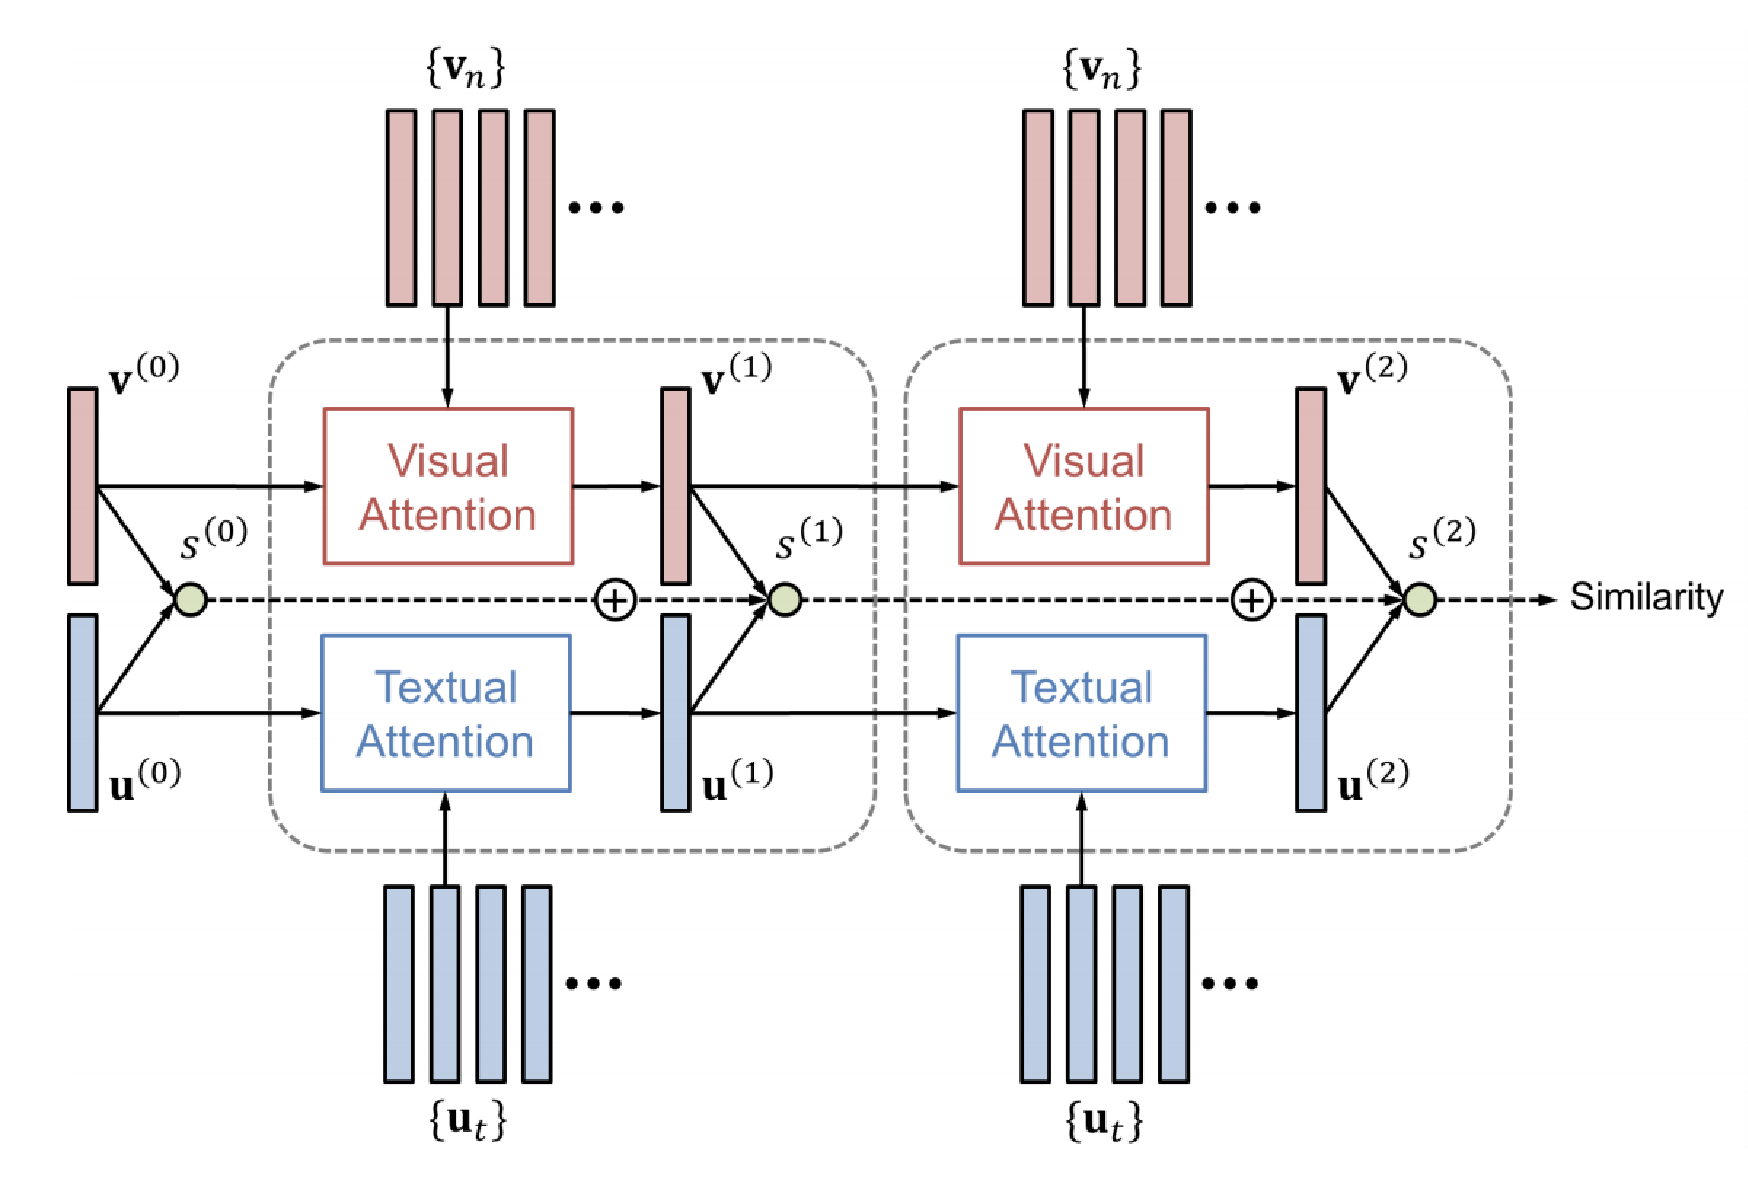
\includegraphics[width=0.8\textwidth]{dan3.pdf}
\caption{m-DAN in case of $\mathbf{K}=2$ \cite{dan}}
\label{fig:dan3}
\end{figure}

In the final experiment, the author used the same Ranking Loss as in the previous work. One difference is that each step of Attention will generate a matching vector. What is done here is to add all $S$.

\subsection{Summary of Image-Text Alignment Related Works}
Throughout these papers, all models are dealing with graphic and text fusion, that is, multi-modal fusion. One of his most basic starting points is that the encoder models for text and images must be good enough, which is the first one, convolution in the article (it seems that Recurrent neural network can also be used).

With an excellent encoder, the next thing to do is the fusion of features. Currently, there are two ways to fuse features, one is pre-fusion, and the other is post-fusion. Pre-fusion inputs image information and text information to a network for further encoder, and finally uses the task-related network; post-fusion is to directly concate the features from the image text encoder and then input to the task-related network. Generally speaking, pre-converged networks are better than post-converged.

Graphic matching is a matching problem of all sentences and all images. It may be relatively tricky to solve this problem directly, so sometimes it is necessary to split these data into components. 

The other is that there are many tricks in the model training. Sometimes or most of the time, it is not because our idea is not good enough, but because we have insufficient experience in training the model, so we tell us that we must be patient in training the model. The road is right, you can keep going, and it will have good results.

\section{Conclusion of Literature}

There are many research focusing on the field of object detection and image-text alignment. We reviewed the research problem and studies their proposed solutions and methodologies. 

In object detection, the major problem is to extract featured object out from images. Convolutional neural network (CNN) \cite{cnn1} was firstly proposed and became the basis of most of the preceding improved models in the field. There are classic deep learning models like VGG \cite{vgg16} and RCNN \cite{rcnn}, followed by more recently improved ones like Fast RCNN \cite{fastrcnn} and Faster RCNN \cite{fasterrcnn}. These deep learning models significantly helped solve the task of object detection and they can achieve promising results.

For image-text alignment, the primary focus is how to map both image and text to the same semantic space. There are CNN models which was able to apply the convolution operation to text such as m-CNN. Recently, models like DAN focus on applying attention mechanism on neural networks to align different image regions to different text tokens, which greatly improved the quality of image-text alignment. 




%%% Local Variables: 
%%% mode: latex
%%% TeX-master: "thesis"
%%% End: 